% Options for packages loaded elsewhere
\PassOptionsToPackage{unicode}{hyperref}
\PassOptionsToPackage{hyphens}{url}
%
\documentclass[
  11pt,
  ignorenonframetext,
]{beamer}
\usepackage{pgfpages}
\setbeamertemplate{caption}[numbered]
\setbeamertemplate{caption label separator}{: }
\setbeamercolor{caption name}{fg=normal text.fg}
\beamertemplatenavigationsymbolsempty
% Prevent slide breaks in the middle of a paragraph
\widowpenalties 1 10000
\raggedbottom
\setbeamertemplate{part page}{
  \centering
  \begin{beamercolorbox}[sep=16pt,center]{part title}
    \usebeamerfont{part title}\insertpart\par
  \end{beamercolorbox}
}
\setbeamertemplate{section page}{
  \centering
  \begin{beamercolorbox}[sep=12pt,center]{part title}
    \usebeamerfont{section title}\insertsection\par
  \end{beamercolorbox}
}
\setbeamertemplate{subsection page}{
  \centering
  \begin{beamercolorbox}[sep=8pt,center]{part title}
    \usebeamerfont{subsection title}\insertsubsection\par
  \end{beamercolorbox}
}
\AtBeginPart{
  \frame{\partpage}
}
\AtBeginSection{
  \ifbibliography
  \else
    \frame{\sectionpage}
  \fi
}
\AtBeginSubsection{
  \frame{\subsectionpage}
}
\usepackage{amsmath,amssymb}
\usepackage{iftex}
\ifPDFTeX
  \usepackage[T1]{fontenc}
  \usepackage[utf8]{inputenc}
  \usepackage{textcomp} % provide euro and other symbols
\else % if luatex or xetex
  \usepackage{unicode-math} % this also loads fontspec
  \defaultfontfeatures{Scale=MatchLowercase}
  \defaultfontfeatures[\rmfamily]{Ligatures=TeX,Scale=1}
\fi
\usepackage{lmodern}
\usetheme[]{Boadilla}
\ifPDFTeX\else
  % xetex/luatex font selection
\fi
% Use upquote if available, for straight quotes in verbatim environments
\IfFileExists{upquote.sty}{\usepackage{upquote}}{}
\IfFileExists{microtype.sty}{% use microtype if available
  \usepackage[]{microtype}
  \UseMicrotypeSet[protrusion]{basicmath} % disable protrusion for tt fonts
}{}
\makeatletter
\@ifundefined{KOMAClassName}{% if non-KOMA class
  \IfFileExists{parskip.sty}{%
    \usepackage{parskip}
  }{% else
    \setlength{\parindent}{0pt}
    \setlength{\parskip}{6pt plus 2pt minus 1pt}}
}{% if KOMA class
  \KOMAoptions{parskip=half}}
\makeatother
\usepackage{xcolor}
\newif\ifbibliography
\usepackage{color}
\usepackage{fancyvrb}
\newcommand{\VerbBar}{|}
\newcommand{\VERB}{\Verb[commandchars=\\\{\}]}
\DefineVerbatimEnvironment{Highlighting}{Verbatim}{commandchars=\\\{\}}
% Add ',fontsize=\small' for more characters per line
\usepackage{framed}
\definecolor{shadecolor}{RGB}{242,242,248}
\newenvironment{Shaded}{\begin{snugshade}}{\end{snugshade}}
\newcommand{\AlertTok}[1]{\textcolor[rgb]{0.94,0.16,0.16}{#1}}
\newcommand{\AnnotationTok}[1]{\textcolor[rgb]{0.56,0.35,0.01}{\textbf{\textit{#1}}}}
\newcommand{\AttributeTok}[1]{\textcolor[rgb]{0.13,0.29,0.53}{#1}}
\newcommand{\BaseNTok}[1]{\textcolor[rgb]{0.00,0.00,0.81}{#1}}
\newcommand{\BuiltInTok}[1]{#1}
\newcommand{\CharTok}[1]{\textcolor[rgb]{0.31,0.60,0.02}{#1}}
\newcommand{\CommentTok}[1]{\textcolor[rgb]{0.56,0.35,0.01}{\textit{#1}}}
\newcommand{\CommentVarTok}[1]{\textcolor[rgb]{0.56,0.35,0.01}{\textbf{\textit{#1}}}}
\newcommand{\ConstantTok}[1]{\textcolor[rgb]{0.56,0.35,0.01}{#1}}
\newcommand{\ControlFlowTok}[1]{\textcolor[rgb]{0.13,0.29,0.53}{\textbf{#1}}}
\newcommand{\DataTypeTok}[1]{\textcolor[rgb]{0.13,0.29,0.53}{#1}}
\newcommand{\DecValTok}[1]{\textcolor[rgb]{0.00,0.00,0.81}{#1}}
\newcommand{\DocumentationTok}[1]{\textcolor[rgb]{0.56,0.35,0.01}{\textbf{\textit{#1}}}}
\newcommand{\ErrorTok}[1]{\textcolor[rgb]{0.64,0.00,0.00}{\textbf{#1}}}
\newcommand{\ExtensionTok}[1]{#1}
\newcommand{\FloatTok}[1]{\textcolor[rgb]{0.00,0.00,0.81}{#1}}
\newcommand{\FunctionTok}[1]{\textcolor[rgb]{0.13,0.29,0.53}{\textbf{#1}}}
\newcommand{\ImportTok}[1]{#1}
\newcommand{\InformationTok}[1]{\textcolor[rgb]{0.56,0.35,0.01}{\textbf{\textit{#1}}}}
\newcommand{\KeywordTok}[1]{\textcolor[rgb]{0.13,0.29,0.53}{\textbf{#1}}}
\newcommand{\NormalTok}[1]{#1}
\newcommand{\OperatorTok}[1]{\textcolor[rgb]{0.81,0.36,0.00}{\textbf{#1}}}
\newcommand{\OtherTok}[1]{\textcolor[rgb]{0.56,0.35,0.01}{#1}}
\newcommand{\PreprocessorTok}[1]{\textcolor[rgb]{0.56,0.35,0.01}{\textit{#1}}}
\newcommand{\RegionMarkerTok}[1]{#1}
\newcommand{\SpecialCharTok}[1]{\textcolor[rgb]{0.81,0.36,0.00}{\textbf{#1}}}
\newcommand{\SpecialStringTok}[1]{\textcolor[rgb]{0.31,0.60,0.02}{#1}}
\newcommand{\StringTok}[1]{\textcolor[rgb]{0.31,0.60,0.02}{#1}}
\newcommand{\VariableTok}[1]{\textcolor[rgb]{0.00,0.00,0.00}{#1}}
\newcommand{\VerbatimStringTok}[1]{\textcolor[rgb]{0.31,0.60,0.02}{#1}}
\newcommand{\WarningTok}[1]{\textcolor[rgb]{0.56,0.35,0.01}{\textbf{\textit{#1}}}}
\usepackage{longtable,booktabs,array}
\usepackage{calc} % for calculating minipage widths
\usepackage{caption}
% Make caption package work with longtable
\makeatletter
\def\fnum@table{\tablename~\thetable}
\makeatother
\usepackage{graphicx}
\makeatletter
\def\maxwidth{\ifdim\Gin@nat@width>\linewidth\linewidth\else\Gin@nat@width\fi}
\def\maxheight{\ifdim\Gin@nat@height>\textheight\textheight\else\Gin@nat@height\fi}
\makeatother
% Scale images if necessary, so that they will not overflow the page
% margins by default, and it is still possible to overwrite the defaults
% using explicit options in \includegraphics[width, height, ...]{}
\setkeys{Gin}{width=\maxwidth,height=\maxheight,keepaspectratio}
% Set default figure placement to htbp
\makeatletter
\def\fps@figure{htbp}
\makeatother
\usepackage{soul}
\setlength{\emergencystretch}{3em} % prevent overfull lines
\providecommand{\tightlist}{%
  \setlength{\itemsep}{0pt}\setlength{\parskip}{0pt}}
\setcounter{secnumdepth}{-\maxdimen} % remove section numbering
\setbeamertemplate{itemize item}[circle]
\setbeamertemplate{enumerate item}[circle]
%\usepackage{layout}    % add `\layout` to the document to show page layout and parameter values
\usepackage{tikz}
\usetikzlibrary{arrows.meta,calc,tikzmark,fit, positioning}
\AtBeginEnvironment{verbatim}{\small}    % reduce font size in R output
% https://stackoverflow.com/questions/35734525/reduce-space-between-code-chunks-and-code-output-in-rmarkdown-beamer-presentatio
\makeatletter
  \preto{\@verbatim}{\topsep=0pt \partopsep=0pt \itemsep=0pt}
\makeatother
% Set some lengths explicitly, for reproducibility across environments with different defaults
% Using fixed values (without rubber lengths) allows for more predictability in sizes,
%  which is useful for graphical overlays, though it may not be as flexible.
% See p. 145 of "The LaTeX Companion" (2e) for a diagram and explanation of some of these parameters.
\setlength{\partopsep}{0pt}
\setlength{\topsep}{0pt}
% My first instinct is to set \parsep to 0 (so paragraphs in the same item are closer together)
%  and set \itemsep to a rubber value; but the default is the opposite!
%  So all paragraphs are the same distance apart, regardless of item number...
% The \tightlist command sets \itemsep and \parskip to 0, but does not change \parsep.
\setlength{\parsep}{6pt plus2pt minus2pt}
\setlength{\itemsep}{0pt}
% For the most part, I don't actually want any space around the Shaded environments,
%  but it's the easiest way I found to reliably reserve space above the code chunks in columns underneath code output (verbatim).
\setlength{\OuterFrameSep}{4pt}  % = \topsep by default in `framed` package (but this is only applied at the start of the environment: the default value of \OuterFrameSep is otherwise \maxdimen!)
\newlength\ShadedFrameSep 
\ifdim\OuterFrameSep=\maxdimen 
  \ShadedFrameSep=\topsep \else 
  \ShadedFrameSep=\OuterFrameSep 
\fi
\newcommand{\ctop}{\vspace{\ShadedFrameSep}}  % for aligning text with the top of a code block in a table (0.2\baselinesep seemed like a good approximation, depending on other parametes; '\topsep+\parskip+\partopsep' seemed logical, but might be too much, maybe because it loses the rubber values)
\newcommand{\Rlogo}{\includegraphics[height=1em]{/Library/Frameworks/R.framework/Resources/doc/html/logo.jpg}}
\newcommand{\R}{\texttt{R}}
\newcommand{\highlight}[1]{\StringTok{#1}}
\newcommand{\important}[1]{\AlertTok{#1}}
\newcommand{\fade}[1]{\textcolor[rgb]{0.66,0.66,0.66}{#1}}
\newcommand{\annote}[1]{{\footnotesize #1}}
\newcommand{\name}[1]{\VariableTok{\texttt{#1}}}
\ifLuaTeX
  \usepackage{selnolig}  % disable illegal ligatures
\fi
\IfFileExists{bookmark.sty}{\usepackage{bookmark}}{\usepackage{hyperref}}
\IfFileExists{xurl.sty}{\usepackage{xurl}}{} % add URL line breaks if available
\urlstyle{same}
\hypersetup{
  pdftitle={A Gentle Introduction to R},
  pdfauthor={Jonathan Whiteley},
  hidelinks,
  pdfcreator={LaTeX via pandoc}}

\title{A Gentle Introduction to R}
\author{Jonathan Whiteley}
\date{2023-08-14}

\begin{document}
\frame{\titlepage}

\begin{frame}[fragile]{Debugging}
\protect\hypertarget{debugging}{}
\small

\texttt{\textbackslash{}baselineskip}: \(\the\baselineskip\) \hfill
\texttt{\textbackslash{}lineskip}: \(\the\lineskip\)\\
\texttt{\textbackslash{}parskip}: \(\the\parskip\) \hfill
\texttt{\textbackslash{}parsep}: \(\the\parsep\)\\
\texttt{\textbackslash{}itemsep}: \(\the\itemsep\) \hfill
\texttt{\textbackslash{}topsep}: \(\the\topsep\)\\
\texttt{\textbackslash{}partopsep}: \(\the\partopsep\) \hfill
\texttt{\textbackslash{}OuterFrameSep}: \(\the\OuterFrameSep\)

\begin{columns}[T]
\begin{column}{0.5\textwidth}
\texttt{\textbackslash{}baselineskip}: \(\the\baselineskip\)\\
\texttt{\textbackslash{}parskip}: \(\the\parskip\)\\
\texttt{\textbackslash{}parsep}: \(\the\parsep\)\\
\texttt{\textbackslash{}itemsep}: \(\the\itemsep\)\\
\texttt{\textbackslash{}topsep}: \(\the\topsep\)\\
\texttt{\textbackslash{}partopsep}: \(\the\partopsep\)\\
\texttt{\textbackslash{}OuterFrameSep}: \(\the\OuterFrameSep\)
\end{column}

\begin{column}{0.5\textwidth}
\begin{Shaded}
baselineskip: \the\baselineskip  \\
parskip: \the\parskip  \\
parsep: \the\parsep  \\
itemsep: \the\itemsep  \\
topsep: \the\topsep \\
partopsep: \the\partopsep \\
OuterFrameSep: \the\OuterFrameSep \\
\end{Shaded}
\end{column}
\end{columns}

\begin{verbatim}
pandoc version: 3.1.1
\end{verbatim}

\begin{verbatim}
knitr version: 1.43
rmarkdown version: 2.23
\end{verbatim}
\end{frame}

\begin{frame}{Prerequisites}
\protect\hypertarget{prerequisites}{}
\begin{itemize}
\item
  Access to a copy of the
  \href{https://www.r-project.org}{\(\includegraphics[height=1em]{/Library/Frameworks/R.framework/Resources/doc/html/logo.jpg}\)}\footnote<.->{The
    R logo
    (\(\includegraphics[height=1em]{/Library/Frameworks/R.framework/Resources/doc/html/logo.jpg}\))
    is \href{https://www.r-project.org/logo/}{© 2016 The R Foundation}
    and used as-is under the terms of the
    \href{https://creativecommons.org/licenses/by-sa/4.0/}{\textbf{CC-BY-SA
    4.0} license}} software

  \begin{itemize}
  \item
    i.e., a ``binary executable''
  \item
    Go to \emph{\href{https://www.r-project.org}{www.r-project.org}} to
    get a copy,\\
    or ask your system administrator.
  \end{itemize}
\item
  Knowledge of common mathematical operations: arithmetic, logarithms,
  etc.
\item
  No previous experience with R or programming required.
\end{itemize}
\end{frame}

\hypertarget{welcome}{%
\section{Welcome}\label{welcome}}

\begin{frame}{Pop Quiz}
\protect\hypertarget{pop-quiz}{}
{\footnotesize \textcolor[rgb]{0.66,0.66,0.66}{We will review these \textit{at the end}, so you can see how much you have learned.}}

\begin{itemize}
\tightlist
\item
  What does `CRAN' stand for?
\item
  Why is it named `\(\texttt{R}\)'?
\item
  How can you use \(\texttt{R}\) \emph{interactively}?
\item
  How do you find out what a function does \& how to use it?
\item
  How do you store values to re-use later?
\item
  True or False: Warnings can be ignored, but an Error means I made a
  mistake.
\item
  True or False: Error messages will tell me how to fix the problem.
\end{itemize}

~

\begin{block}{Answer in the chat:}
\protect\hypertarget{answer-in-the-chat}{}
What emoji best describes your current mood or state of mind?
\end{block}
\end{frame}

\begin{frame}[fragile]{Introductions}
\protect\hypertarget{introductions}{}
\begin{itemize}
\tightlist
\item
  Name
\item
  Pronouns
\item
  Job title, role
\item
  \emph{optional}: a hobby or activity you enjoy?
\end{itemize}

\begin{itemize}
\tightlist
\item
  Have you used \(\texttt{R}\) before?
\item
  Have you used a programming language before?
\end{itemize}

\note{Other icebreaker questions:

\begin{itemize}
\tightlist
\item
  Favourite candy or treat as a child?
\item
  Favourite music band or genre?
\item
  Favourite book?
\item
  Highlight of the past month / year (personal or professional)?
\end{itemize}

If available on platform, online polls:

\begin{itemize}
\tightlist
\item
  Where are you joining from?
\item
  Have you used \texttt{R} before?
\item
  Have you used a programming language before?
\end{itemize}

If a chat is available, put answer to a question there:

\begin{itemize}
\tightlist
\item
  What emoji best describes your current mood or state of mind?
\item
  Favourite emoji?
\end{itemize}

More icebreaker ideas:

\begin{itemize}
\tightlist
\item
  \url{https://blog.slido.com/virtual-icebreakers/}
\item
  \url{https://www.mural.co/blog/virtual-meeting-ice-breakers}
\end{itemize}}
\end{frame}

\begin{frame}{ Icebreaker activity}
\protect\hypertarget{icebreaker-activity}{}
\begin{columns}[T,onlytextwidth]
\begin{column}{0.48\textwidth}
\textbf{What is this?}\\
1--3 word description, for~example:

\begin{itemize}
\tightlist
\item
  ``This is grey''
\item
  ``This looks uncomfortable''
\end{itemize}

\textbf{OR} caption this image?

\hfill\break
On your turn:

\begin{enumerate}
\item
  Previous person's name
\item
  Their answer to the question
\item
  Your name
\item
  Your answer
\item
  Name of the person to go next
\end{enumerate}
\end{column}

\begin{column}{0.5\textwidth}
\begin{figure}
\centering
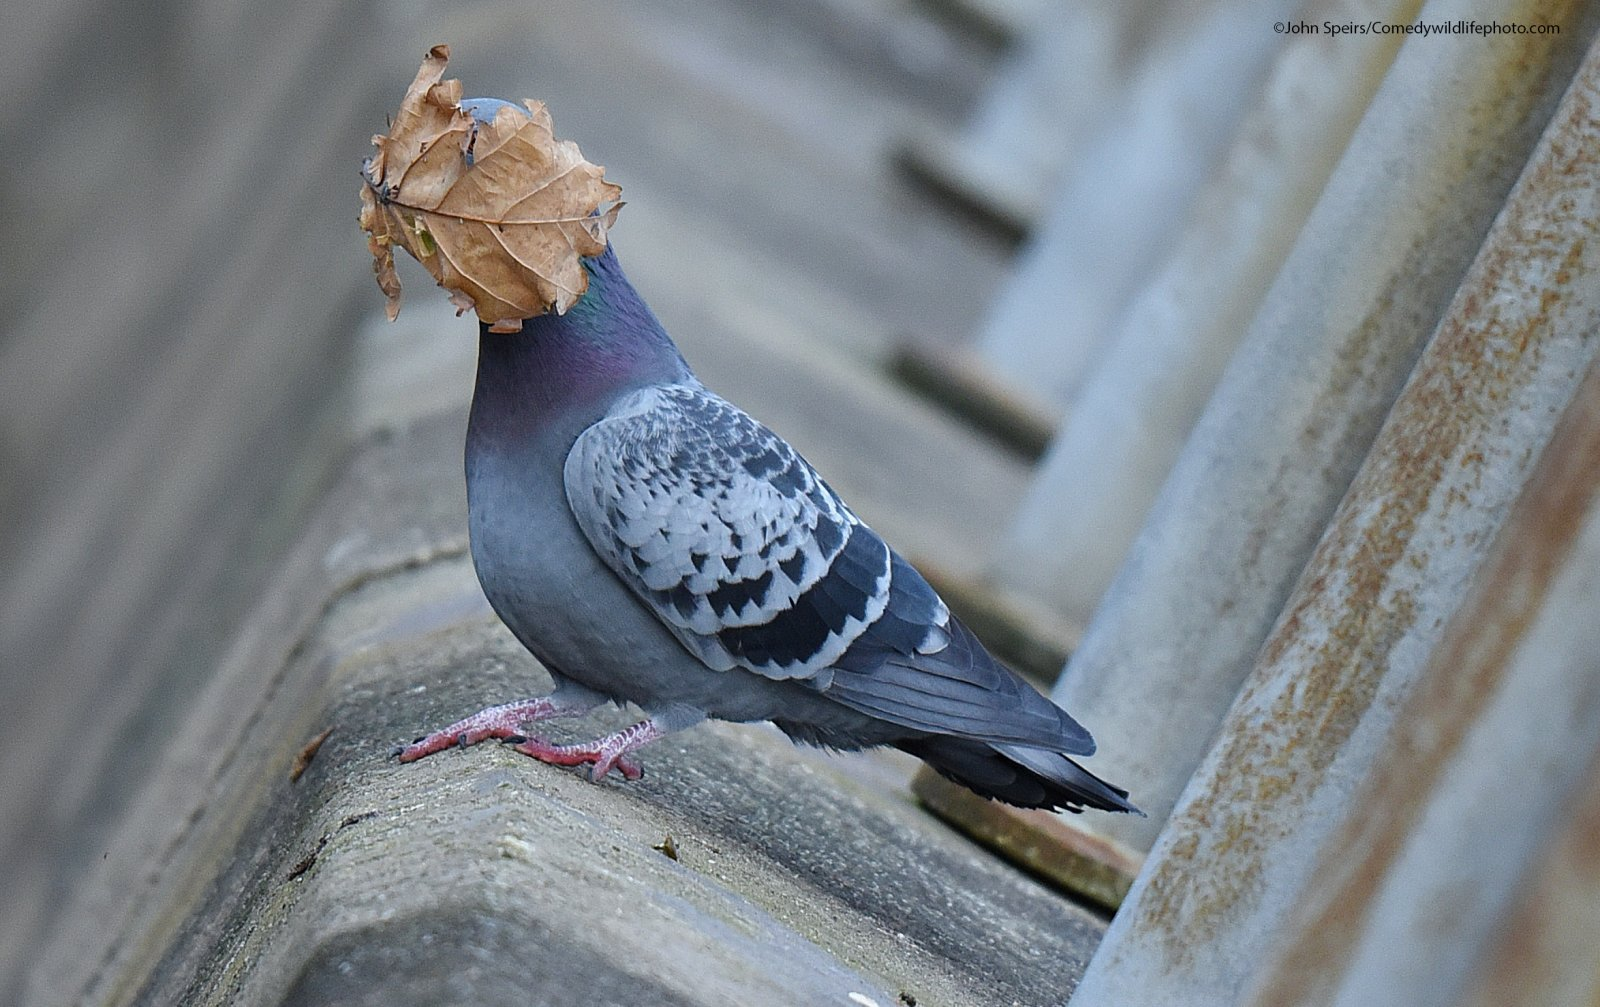
\includegraphics[width=1\textwidth,height=\textheight]{images/john-speirs_i-guess-summers-over.jpg}
\caption{Caption this image.\\
©~\href{https://www.comedywildlifephoto.com/gallery/comedy-wildlife-2021-competition-winners.php}{John~Speirs/\linebreak[0]Comedywildlifephoto.com}}
\end{figure}
\end{column}
\end{columns}
\end{frame}

\begin{frame}{Learning Objectives}
\protect\hypertarget{learning-objectives}{}
\begin{itemize}
\tightlist
\item
  Get familiar with the
  \includegraphics[width=\textwidth,height=1em]{/Library/Frameworks/R.framework/Resources/doc/html/logo.jpg}
  \emph{interface}
\item
  Use technical \emph{terms} for \(\texttt{R}\) concepts
\item
  Enter \emph{commands}

  \begin{itemize}
  \tightlist
  \item
    use \(\texttt{R}\) interactively: understand input \& output
  \item
    use some common \emph{functions}
  \end{itemize}
\item
  Get familiar with `\(\texttt{R}\) objects'

  \begin{itemize}
  \tightlist
  \item
    store \& retrieve values
  \end{itemize}
\item
  Understand \emph{Errors}, \emph{Warnings}, and \emph{Messages}
\item
  How to get Help
\end{itemize}
\end{frame}

\begin{frame}[fragile]{Why is it named `\(\texttt{R}\)'?}
\protect\hypertarget{why-is-it-named-textttr}{}
\begin{enumerate}
\item
  \textbf{\(\texttt{R}\)} started as an \emph{open-source}
  implementation of the\\
  \textbf{\texttt{S}} statistical computing language
  (S-PLUS)\footnote<.->{\url{https://www.r-project.org/about.html}}

  \begin{itemize}
  \item
    \texttt{S} was created at Bell Laboratories in 1976\footnote<.->{\url{https://en.wikipedia.org/wiki/S_(programming_language)}}
  \item
    \(\texttt{R}\) was based on the \texttt{S} syntax (mostly v3), but
    works very differently ``under the hood''.
  \end{itemize}
\item
  \textbf{\(\texttt{R}\)} was created by \ul{\textbf{R}}oss Ihaka and
  \ul{\textbf{R}}obert Gentleman --- aka ``R \& R''\footnote<.->{\url{https://www.r-project.org/contributors.html}}
  --- at the University of Aukland in the early 1990s.
\end{enumerate}

\bigskip

\emph{Read more about the history of \(\texttt{R}\) on
\href{https://en.wikipedia.org/wiki/R_(programming_language)\#History}{Wikipedia}}\footnote<.->{\url{https://en.wikipedia.org/wiki/R_(programming_language)\#History}}
\end{frame}

\hypertarget{interacting-with-textttr-interface}{%
\section{\texorpdfstring{Interacting with \(\texttt{R}\)
(Interface)}{Interacting with \textbackslash texttt\{R\} (Interface)}}\label{interacting-with-textttr-interface}}

\begin{frame}{The
\(\includegraphics[height=1em]{/Library/Frameworks/R.framework/Resources/doc/html/logo.jpg}\)
Interface}
\protect\hypertarget{the-includegraphicsheight1emlibraryframeworksr.frameworkresourcesdochtmllogo.jpg-interface}{}
\begin{itemize}
\tightlist
\item
  `base \(\texttt{R}\)' has a slightly different interface for each
  \textbf{O}perating \textbf{S}ystem (OS)

  \begin{itemize}
  \tightlist
  \item
    GUI = \textbf{G}raphical \textbf{U}ser \textbf{I}nterface
  \end{itemize}
\item
  \(\texttt{R}\) can also run inside of a terminal (no GUI) or other
  software (different GUI).
\end{itemize}

\begin{block}{\href{https://en.wikipedia.org/wiki/Integrated_development_environment}{\textbf{I}ntegrated
\textbf{D}evelopment \textbf{E}nvironment} (IDE)}
\protect\hypertarget{integrated-development-environment-ide}{}
\begin{itemize}
\tightlist
\item
  An IDE is like an extra interface layer on top of `base
  \(\texttt{R}\)'
\item
  IDEs often add convenient tools to make writing code easier (e.g.,
  syntax highlighting), and for developing larger projects with multiple
  files.
\item
  \textbf{\href{https://posit.co/products/open-source/rstudio/}{RStudio}}
  is one of the most popular cross-platform IDEs for \(\texttt{R}\).

  \begin{itemize}
  \tightlist
  \item
    RStudio is available in open source (free/libre) and
    commercial\footnote<.->{for organizations not able to use software
      licensed with AGPL} editions.
  \end{itemize}
\end{itemize}
\end{block}
\end{frame}

\begin{frame}{A quick tour of the `base \(\texttt{R}\) GUI'}
\protect\hypertarget{a-quick-tour-of-the-base-textttr-gui}{}
\begin{figure}
\centering
\begin{tikzpicture}[overlay/.style={ultra thick, rounded corners, draw=red, fill=white, fill opacity=0.5, text opacity=1},
                    note/.style={align=center, font=\Large\bfseries}]
  \node[anchor=south west,inner sep=0] (image) at (0,0) {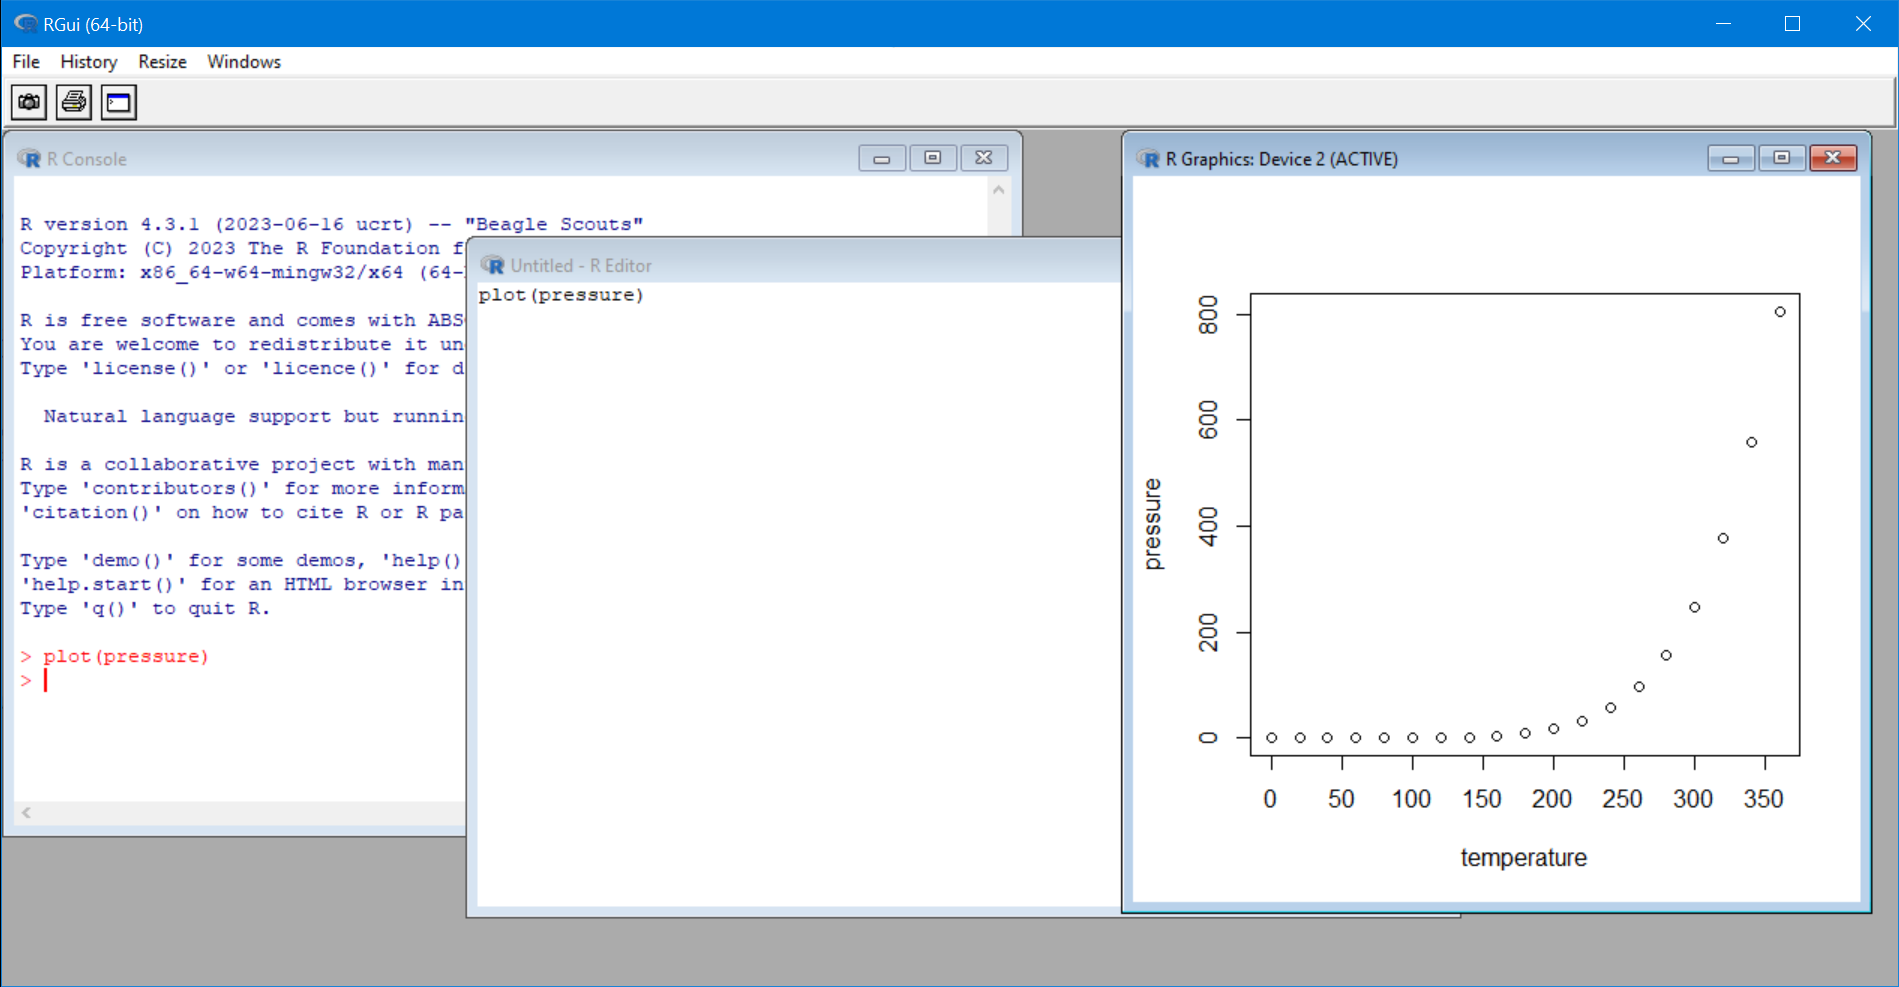
\includegraphics[width=0.9\textwidth]{images/R-screenshot-script-plot-win.png}};
  \begin{scope}[x={(image.south east)},y={(image.north west)}]
    \draw[overlay] (0,0.15) rectangle (0.54,0.87);
    \node[note] at (0.14,0.27) {console};
    \draw[overlay] (0.245,0.065) rectangle (0.585,0.76);
    \node[note] at (0.415,0.41) {source};
    \draw[overlay] (0.588,0.07) rectangle (0.987,0.87);
    \node[note] at (0.788,0.47) {plot\\ window};
  \end{scope}
\end{tikzpicture}
\caption{Screenshot of the R GUI in Windows.}
\end{figure}
\end{frame}

\begin{frame}{A quick tour of RStudio}
\protect\hypertarget{a-quick-tour-of-rstudio}{}
\begin{columns}[T,onlytextwidth]
\begin{column}{0.73\textwidth}
The RStudio GUI has 4 `panes' that contain `tabs'.

\begin{figure}
\centering
\begin{tikzpicture}[overlay/.style={ultra thick, draw=red, fill=white, fill opacity=0.5, text opacity=1},
                    circler/.style={radius=3ex},
                    note/.style={align=center, font=\Large\bfseries}]
  \node[anchor=south west,inner sep=0] (image) at (0,0) {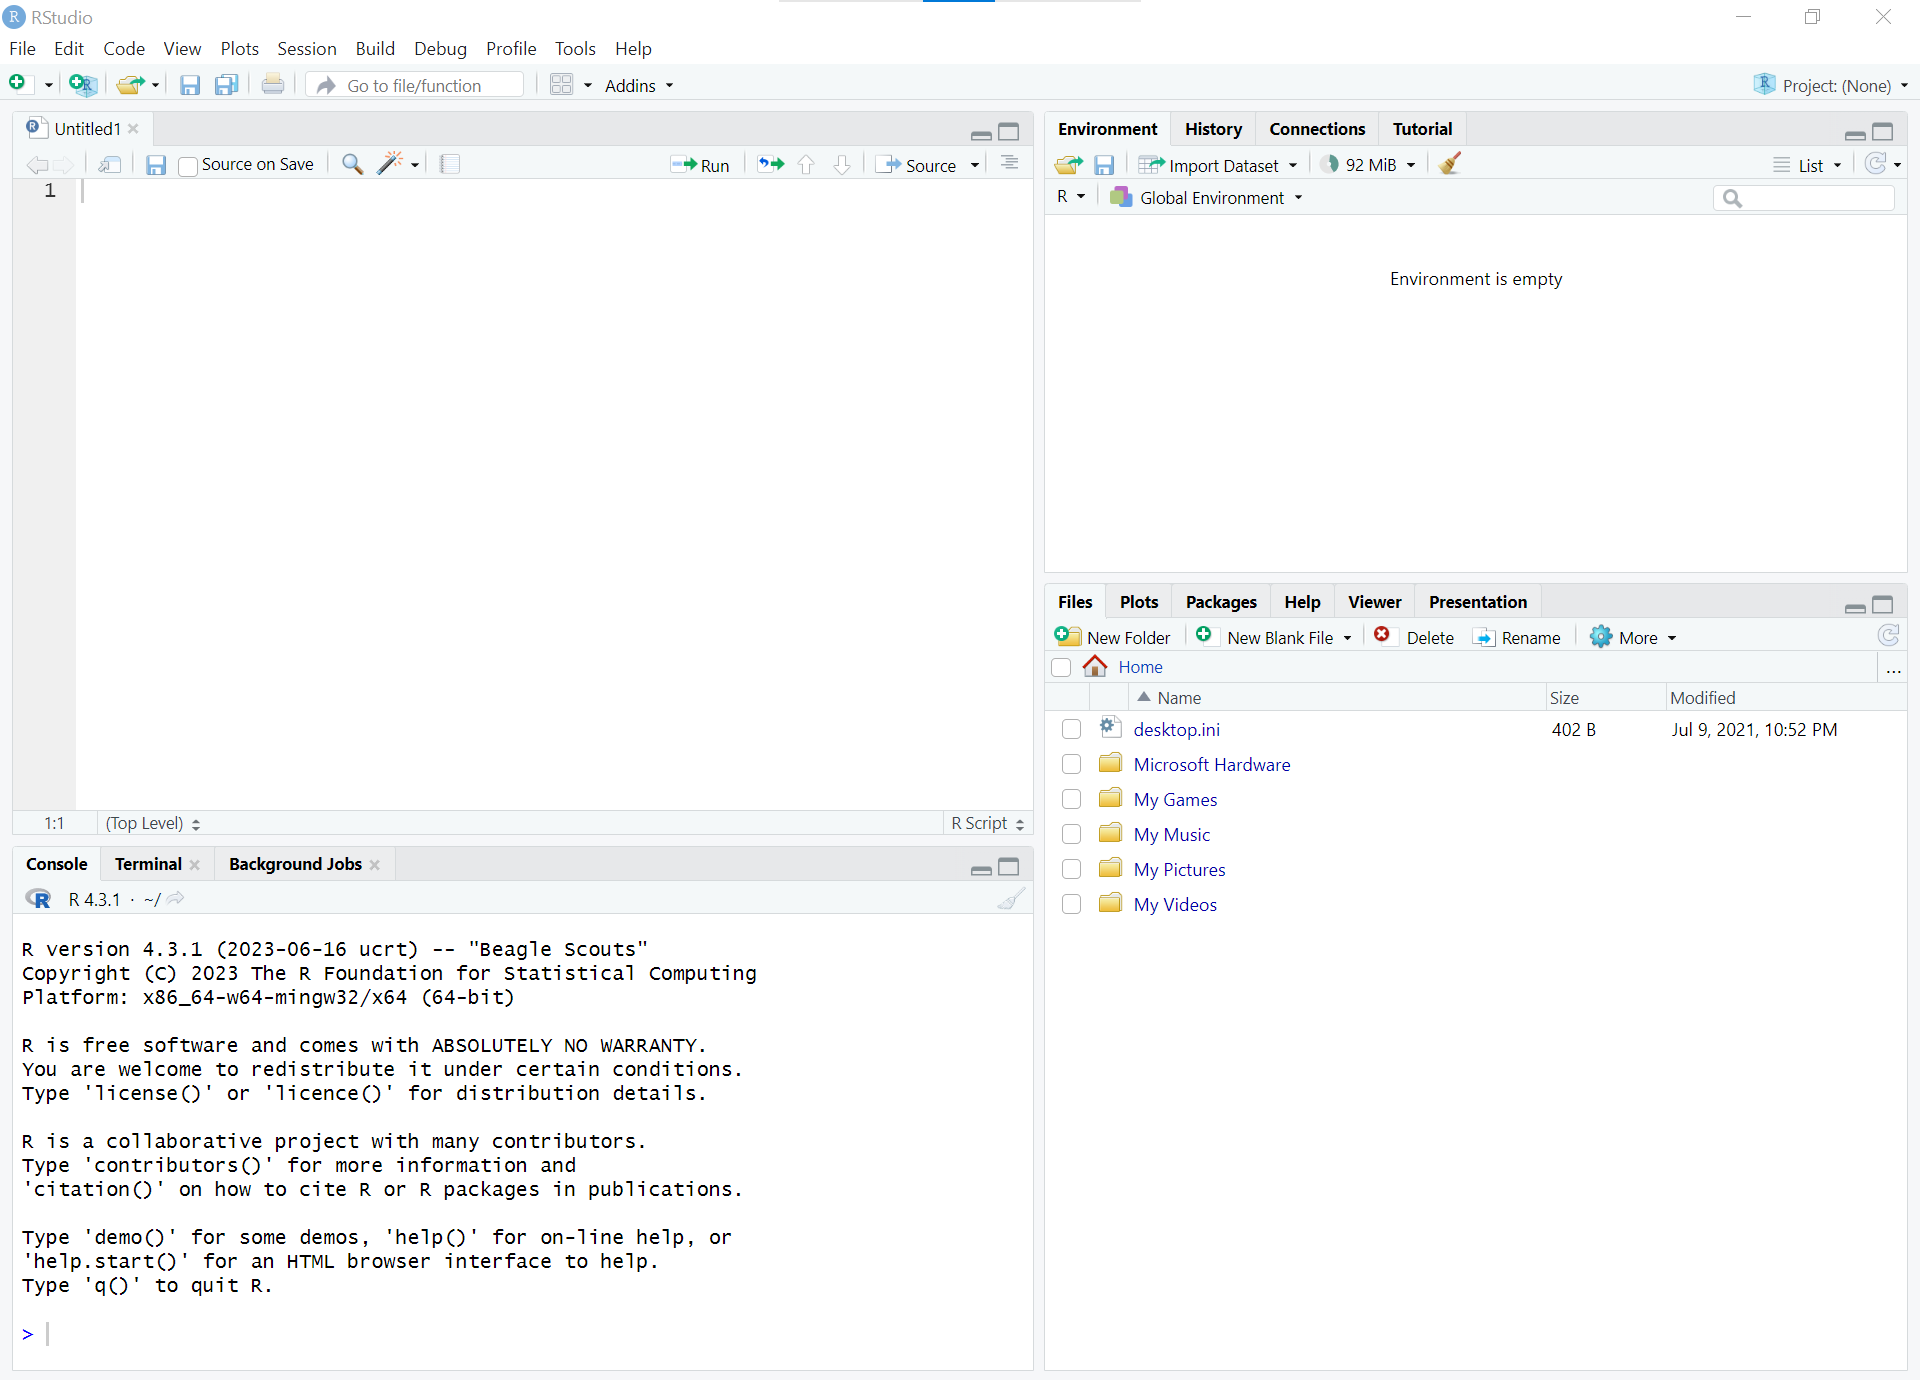
\includegraphics[width=\textwidth]{images/RStudio-screenshot-4pane-default.png}};
  \begin{scope}[x={(image.south east)},y={(image.north west)}]
    \draw[overlay] (0.45,0.7) circle[circler] node[note] {1};
    \draw[overlay] (0.45,0.2) circle[radius=3ex] node[note] {2};
    \draw[overlay] (0.80,0.7) circle[radius=3ex] node[note] {3};
    \draw[overlay] (0.80,0.2) circle[radius=3ex] node[note] {4};
  \end{scope}
\end{tikzpicture}
\caption{Screenshot of RStudio (default layout).}
\end{figure}
\end{column}

\begin{column}{0.25\textwidth}
left:

\begin{enumerate}
\item
  top: \textbf{Source}\footnote<.->{empty until you create or open a
    file}
\item
  bottom: \textbf{Console, Terminal, \ldots{}}
\end{enumerate}

right:

\begin{enumerate}
\setcounter{enumi}{2}
\item
  top:\\
  \textbf{Environment, History, \ldots{}}
\item
  bottom: \textbf{Files, Plots, Help, \ldots{}}
\end{enumerate}
\end{column}
\end{columns}
\end{frame}

\begin{frame}{Interacting with
\(\includegraphics[height=1em]{/Library/Frameworks/R.framework/Resources/doc/html/logo.jpg}\)}
\protect\hypertarget{interacting-with-includegraphicsheight1emlibraryframeworksr.frameworkresourcesdochtmllogo.jpg}{}
\begin{itemize}
\item
  Regardless of the GUI, you interact with \(\texttt{R}\) primarily
  using a \emph{command~line}

  \begin{itemize}
  \tightlist
  \item
    aka a \ul{c}ommand \ul{l}ine \ul{i}nterface (cli)
  \item
    the command line is usually in the \emph{console}
  \end{itemize}
\item
  ``Question-and-Answer Model''

  \begin{itemize}
  \item
    You ask \(\texttt{R}\) to do something (a \emph{command}),\\
    \hspace*{0.333em}\hspace*{0.333em}\hspace*{0.333em}\hspace*{0.333em}\hspace*{0.333em}and
    \(\texttt{R}\) tells you the answer (\emph{result}).
  \end{itemize}
\item
  Instructions are given to \(\texttt{R}\) using the \emph{R language}.
\end{itemize}

\note{R is designed so that users can start by using it
\emph{interactively} (what we will do today), and then gradually use it
for more programming as their needs and skills grow.

\begin{itemize}
\tightlist
\item
  Not ``point-and-click'': no menus or wizards to guide you through
  steps of an analysis or procedure.
\end{itemize}}
\end{frame}

\begin{frame}[fragile]{The
\(\includegraphics[height=1em]{/Library/Frameworks/R.framework/Resources/doc/html/logo.jpg}\)
console}
\protect\hypertarget{the-includegraphicsheight1emlibraryframeworksr.frameworkresourcesdochtmllogo.jpg-console}{}
The \emph{console} is a window or pane where you will find:

\begin{itemize}
\item
  The \emph{command line}

  \begin{itemize}
  \tightlist
  \item
    where you will enter commands for \(\texttt{R}\) to run
  \end{itemize}
\item
  Results of commands and other output
\item
  \texttt{Messages}, \WarningTok{Warnings}, and \ErrorTok{Errors}
\end{itemize}
\end{frame}

\begin{frame}[fragile]{The
\(\includegraphics[height=1em]{/Library/Frameworks/R.framework/Resources/doc/html/logo.jpg}\)
command-line}
\protect\hypertarget{the-includegraphicsheight1emlibraryframeworksr.frameworkresourcesdochtmllogo.jpg-command-line}{}
\begin{itemize}
\item
  The command \emph{prompt} normally looks like this\footnote<.->{\textcolor[rgb]{0.66,0.66,0.66}{the colour of the prompt varies depending on the interface}}:

\begin{Shaded}
\begin{Highlighting}[]
\NormalTok{\textgreater{}}
\end{Highlighting}
\end{Shaded}

  \begin{itemize}
  \tightlist
  \item
    This is \(\texttt{R}\)'s way of saying ``I am ready to accept new
    commands''.
  \item
    Type a new command on the line after this prompt (i.e.,
    \emph{input}).
  \end{itemize}
\item
  \textbf{Press \AlertTok{\texttt{return}}/\AlertTok{\texttt{enter}} to
  \emph{run} the current \emph{command} }
\item
  If you can still edit the command next to the prompt, then it has not
  been submitted to \(\texttt{R}\) to execute (it is still waiting for
  input).
\item
  If the last prompt is not empty (i.e., there is text beside it)\\
  \emph{and} you cannot edit what is beside the prompt,\\
  it means \(\texttt{R}\) is still running the last command and is not
  ready to accept a new command yet.

  \begin{itemize}
  \tightlist
  \item
    Wait for a new empty prompt to appear before entering the next
    command.
  \end{itemize}
\end{itemize}
\end{frame}

\begin{frame}[fragile]{The
\(\includegraphics[height=1em]{/Library/Frameworks/R.framework/Resources/doc/html/logo.jpg}\)
command-line (continued)}
\protect\hypertarget{the-includegraphicsheight1emlibraryframeworksr.frameworkresourcesdochtmllogo.jpg-command-line-continued}{}
\begin{itemize}
\item
  If the prompt looks like this:

\begin{Shaded}
\begin{Highlighting}[]
\NormalTok{+}
\end{Highlighting}
\end{Shaded}

  it means the last command was \emph{incomplete} and \(\texttt{R}\) is
  waiting for more input.\\
  \(\texttt{R}\) will not do anything until the command is completed or
  cancelled.

  \begin{itemize}
  \tightlist
  \item
    This usually means you forgot a closing\\
    \emph{quote} \AlertTok{\texttt{"}}, \emph{parenthesis}
    \AlertTok{\texttt{(}}, \emph{bracket} \AlertTok{\texttt{[}}, or
    \emph{brace} \AlertTok{\texttt{\{}}
  \end{itemize}
\item
  \StringTok{You can \textit{cancel} the current command at any time by pressing \texttt{escape}}
  (\AlertTok{\texttt{esc}})
\end{itemize}
\end{frame}

\hypertarget{warming-up-some-early-commands}{%
\section{Warming up: some early
commands}\label{warming-up-some-early-commands}}

\begin{frame}[fragile]{Input \& Output}
\protect\hypertarget{input-output}{}
In this presentation,

\begin{itemize}
\item
  \emph{commands} that can be entered in the \emph{command-line} look
  like this:

\hypertarget{format_input}{%
\label{format_input}}%
\begin{Shaded}
\begin{Highlighting}[]
\NormalTok{Input (commands)}
\end{Highlighting}
\end{Shaded}

  \begin{itemize}
  \tightlist
  \item
    You can try these yourself!
  \end{itemize}
\item
  Expected output (results) look like this:

\begin{verbatim}
Output (results)
\end{verbatim}
\end{itemize}
\end{frame}

\begin{frame}{\(\includegraphics[height=1em]{/Library/Frameworks/R.framework/Resources/doc/html/logo.jpg}\)
offers suggestions}
\protect\hypertarget{includegraphicsheight1emlibraryframeworksr.frameworkresourcesdochtmllogo.jpg-offers-suggestions}{}
Read the opening message carefully.

\begin{figure}
\centering
\begin{tikzpicture}[overlay/.style={ultra thick, rounded corners, draw=red, fill=none},
                    note/.style={anchor=west, align=left, font=\Large\bfseries},
                    ->/.style={ultra thick, red, -{Latex}[round]}]
  \node[anchor=south west,inner sep=0] (image) at (0,0) {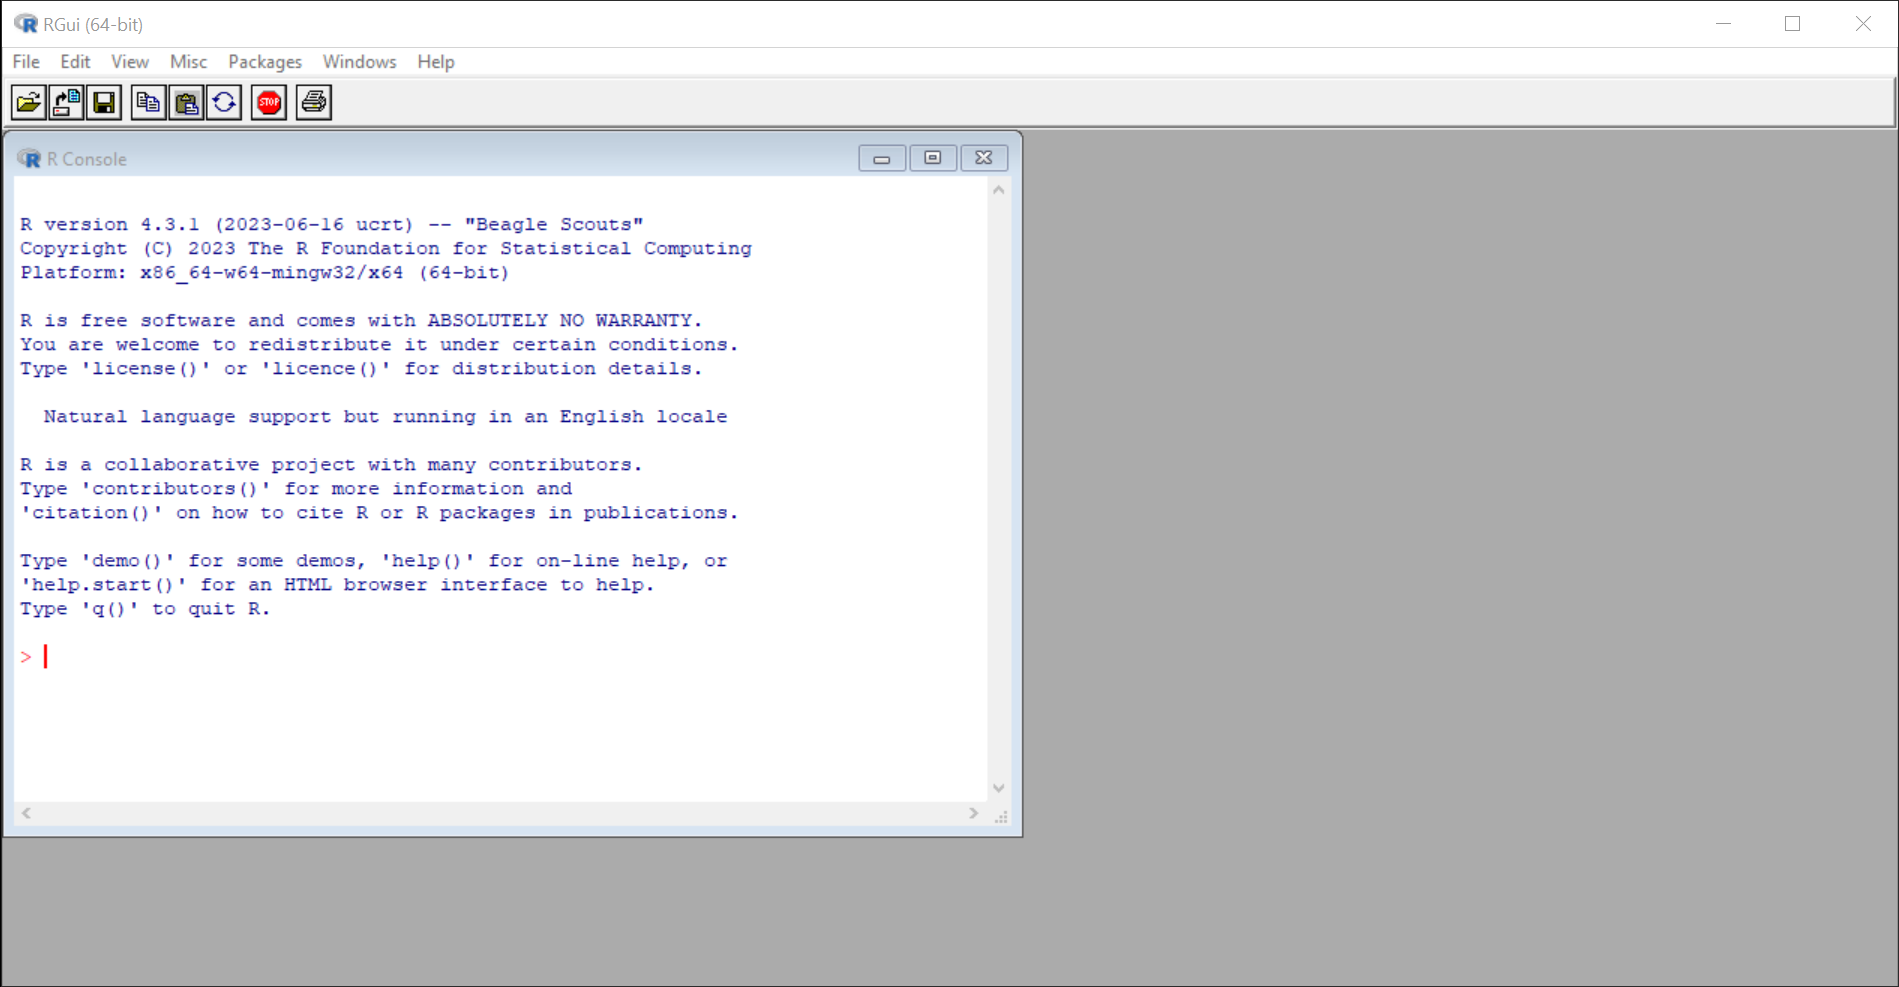
\includegraphics[width=0.9\textwidth]{images/R-screenshot-win-default}};
  \begin{scope}[x={(image.south east)},y={(image.north west)}]
    \node (rect) [overlay, fit={(0,0.36) (0.42,0.46)}, inner sep=0] {};
    \node (note)  [note, text width=12em] at (0.55,0.41) {\textcolor[rgb]{0.60,0.00,0.00}{$\R$ offers suggestions to start with}};
    \draw [->] (note.west) -> (rect.east);
  \end{scope}
\end{tikzpicture}
\caption{$\texttt{R}$ offers suggestions of commands to \KeywordTok{\texttt{Type}} in the console when it starts.}
\end{figure}
\end{frame}

\begin{frame}[fragile]{\(\includegraphics[height=1em]{/Library/Frameworks/R.framework/Resources/doc/html/logo.jpg}\)
is a show-off}
\protect\hypertarget{includegraphicsheight1emlibraryframeworksr.frameworkresourcesdochtmllogo.jpg-is-a-show-off}{}
\begin{longtable}[]{@{}
  >{\raggedright\arraybackslash}p{(\columnwidth - 2\tabcolsep) * \real{0.2625}}
  >{\raggedright\arraybackslash}p{(\columnwidth - 2\tabcolsep) * \real{0.7375}}@{}}
\toprule\noalign{}
\endhead
\begin{minipage}[t]{\linewidth}\raggedright
\begin{Shaded}
\begin{Highlighting}[]
\FunctionTok{demo}\NormalTok{(graphics)}
\end{Highlighting}
\end{Shaded}
\end{minipage} & \begin{minipage}[t]{\linewidth}\raggedright
\begin{itemize}
\tightlist
\item
  some plots and graphs that can be made with \(\texttt{R}\)
\end{itemize}
\end{minipage} \\
\begin{minipage}[t]{\linewidth}\raggedright
\begin{Shaded}
\begin{Highlighting}[]
\FunctionTok{demo}\NormalTok{(image)}
\end{Highlighting}
\end{Shaded}
\end{minipage} & \begin{minipage}[t]{\linewidth}\raggedright
\begin{itemize}
\tightlist
\item
  image-like graphics and maps that can be produced with \(\texttt{R}\)
\end{itemize}
\end{minipage} \\
\begin{minipage}[t]{\linewidth}\raggedright
\begin{Shaded}
\begin{Highlighting}[]
\FunctionTok{demo}\NormalTok{(lm.glm)}
\end{Highlighting}
\end{Shaded}
\end{minipage} & \begin{minipage}[t]{\linewidth}\raggedright
\begin{itemize}
\tightlist
\item
  a demonstration of linear modelling \& GLMs
\end{itemize}
\end{minipage} \\
\begin{minipage}[t]{\linewidth}\raggedright
\begin{Shaded}
\begin{Highlighting}[]
\FunctionTok{demo}\NormalTok{()}
\end{Highlighting}
\end{Shaded}
\end{minipage} & \begin{minipage}[t]{\linewidth}\raggedright
\begin{itemize}
\tightlist
\item
  a list of available demos
\end{itemize}
\end{minipage} \\
\begin{minipage}[t]{\linewidth}\raggedright
\begin{Shaded}
\begin{Highlighting}[]
\FunctionTok{help.start}\NormalTok{()}
\end{Highlighting}
\end{Shaded}
\end{minipage} & \begin{minipage}[t]{\linewidth}\raggedright
\vspace{\ShadedFrameSep}{}

\textbf{←} A great place to start,\\
\hspace*{0.333em}\hspace*{0.333em}\hspace*{0.333em}\hspace*{0.333em}especially
if you are comfortable reading\\
\hspace*{0.333em}\hspace*{0.333em}\hspace*{0.333em}\hspace*{0.333em}documentation
for a programming language.\\
\hspace*{0.333em}\hspace*{0.333em}\hspace*{0.333em}\hspace*{0.333em}More
on this later.
\end{minipage} \\
\bottomrule\noalign{}
\end{longtable}

\begin{block}{Note}
\protect\hypertarget{note}{}
\texttt{R}{} will not only show the output, but also \emph{the code used
to produce it}.
\end{block}
\end{frame}

\begin{frame}[fragile]{\(\includegraphics[height=1em]{/Library/Frameworks/R.framework/Resources/doc/html/logo.jpg}\)
is a calculator}
\protect\hypertarget{includegraphicsheight1emlibraryframeworksr.frameworkresourcesdochtmllogo.jpg-is-a-calculator}{}
\begin{columns}[T,onlytextwidth]
\begin{column}{0.45\textwidth}
\begin{Shaded}
\begin{Highlighting}[]
\DecValTok{1} \SpecialCharTok{+} \DecValTok{1}
\end{Highlighting}
\end{Shaded}

\begin{verbatim}
[1] 2
\end{verbatim}

\begin{Shaded}
\begin{Highlighting}[]
\DecValTok{2} \SpecialCharTok{*} \DecValTok{2}
\end{Highlighting}
\end{Shaded}

\begin{verbatim}
[1] 4
\end{verbatim}

\begin{Shaded}
\begin{Highlighting}[]
\DecValTok{2} \SpecialCharTok{\^{}} \DecValTok{3}
\end{Highlighting}
\end{Shaded}

\begin{verbatim}
[1] 8
\end{verbatim}
\end{column}

\begin{column}{0.45\textwidth}
\begin{Shaded}
\begin{Highlighting}[]
\DecValTok{10} \SpecialCharTok{{-}} \DecValTok{1}
\end{Highlighting}
\end{Shaded}

\begin{verbatim}
[1] 9
\end{verbatim}

\begin{Shaded}
\begin{Highlighting}[]
\DecValTok{8} \SpecialCharTok{/} \DecValTok{2}
\end{Highlighting}
\end{Shaded}

\begin{verbatim}
[1] 4
\end{verbatim}

\begin{Shaded}
\begin{Highlighting}[]
\FunctionTok{sqrt}\NormalTok{(}\DecValTok{9}\NormalTok{)}
\end{Highlighting}
\end{Shaded}

\begin{verbatim}
[1] 3
\end{verbatim}
\end{column}
\end{columns}

\begin{itemize}
\tightlist
\item
  These are \emph{expressions}
\item
  \emph{Expressions} are \emph{evaluated}, and the \emph{value} (result)
  is \emph{returned} (sometimes~\emph{invisibly})
\end{itemize}

\note{The bullet points are accurate, but I note that the
\href{https://cran.r-project.org/doc/manuals/r-release/R-lang.html}{R
Language Definition} distinguishes between `expressions', which are
actually a type of object, and `statements' (see s2.1.3 `Language
objects', s2.1.4 `Expression objects'):

\begin{itemize}
\tightlist
\item
  An \emph{expression} \[object?\] contains one or more statements.
\item
  A statement is a syntactically correct collection of tokens.
\item
  Expression objects are special language objects which contain parsed
  but unevaluated R statements.
\item
  ``an expression object can contain several such expressions'' (not
  clear)
\end{itemize}

Therefore, my understanding is that a \emph{statement} is parsed (by the
R parser), which results in an unevaluated \emph{expression} (an object
of mode ``expression''), which can in turn be evaluated (by `the
evaluator', such as \texttt{eval()}) to return the \emph{value}.

``All expressions have a value.'' (s3 `Evaluation of expressions')}
\end{frame}

\begin{frame}{\(\includegraphics[height=1em]{/Library/Frameworks/R.framework/Resources/doc/html/logo.jpg}\)
command-line tips}
\protect\hypertarget{includegraphicsheight1emlibraryframeworksr.frameworkresourcesdochtmllogo.jpg-command-line-tips}{}
\begin{itemize}
\item
  With the cursor next to the empty prompt (\OtherTok{\texttt{>}}),\\
  use the up \& down \AlertTok{arrow keys} (↑↓) to re-produce previous
  commands.
\item
  This lets you ``scroll through your \emph{command history}''.
\item
  Press \AlertTok{up} (\AlertTok{$\uparrow$}) once, and you get the last
  command you entered\\
  without having to copy \& paste.
\end{itemize}
\end{frame}

\hypertarget{simple-textttr-objects}{%
\section{\texorpdfstring{Simple \(\texttt{R}\)
objects}{Simple \textbackslash texttt\{R\} objects}}\label{simple-textttr-objects}}

\begin{frame}[fragile]{Vectors}
\protect\hypertarget{vectors}{}
\begin{itemize}
\item
  The most basic kind of \emph{object} in \(\texttt{R}\) is a
  \emph{vector}
\item
  Think of a vector as a list of related values (data),\\
  which are \emph{all the same type}
\item
  A single value is an ``\emph{atomic vector}'' (a vector with a length
  of 1)
\end{itemize}

\hfill\break

\begin{columns}[c]
\begin{column}{0.25\textwidth}
\centering
\AlertTok{\Large\textbf{\tikzmarknode{index}{\textit{index}:}\\ the item\\ number}}
\end{column}

\begin{column}{0.5\textwidth}
\hfill\tikzmarknode[anchor=north west, inner sep=0]{code_tr}{}

\begin{verbatim}
[1] 2
\end{verbatim}

\begin{Shaded}
\begin{Highlighting}[]
\DecValTok{1}\SpecialCharTok{:}\DecValTok{10}
\end{Highlighting}
\end{Shaded}

\begin{verbatim}
 [1]  1  2  3  4  5  6  7  8
 [9]  9 10
\end{verbatim}

\tikzmarknode[anchor=north west, inner sep=0]{code_bl}{}\vspace{-\baselineskip}
\end{column}

\begin{column}{0.25\textwidth}
\centering
\AlertTok{\Large\textbf{\tikzmarknode{value}{\textit{value}}}}
\end{column}
\end{columns}

\begin{tikzpicture}[remember picture, overlay, 
                    arr/.style={ultra thick, red, -{Latex}[round]}]
  \node[anchor=south west,inner sep=0, fit={(code_bl)(code_tr)}] (code) {};
  \begin{scope}[shift=(code.south west),x=(code.south east),y=(code.north west)]
    \draw let \p1 = (index.east) in 
      [arr] (index.east) -- (-0.5cm,\y1) -- (-0.5cm,0.88) -> (-0.01,0.88);
    \draw let \p1 = (index.east) in 
      [arr] (index.east) -- (-0.5cm,\y1) -- (-0.5cm,0.37) -> (0.02,0.37);
    \draw let \p1 = (value.west) in 
      [arr] (value.west) -- (0.25,\y1) -- (0.25,0.87) -> (0.18,0.87);
    \draw let \p1 = (value.west) in 
      [arr] (value.west) -- (0.25,\y1) -- (0.21,0.44);
  \end{scope}
\end{tikzpicture}
\end{frame}

\begin{frame}[fragile]{Using vectors}
\protect\hypertarget{using-vectors}{}
\begin{itemize}
\item
  Vectors can be used in calculations
\item
  Operations are applied to each item (\emph{element-wise})

\begin{Shaded}
\begin{Highlighting}[]
\FunctionTok{sum}\NormalTok{( }\FunctionTok{c}\NormalTok{(}\DecValTok{1}\NormalTok{, }\DecValTok{2}\NormalTok{, }\DecValTok{3}\NormalTok{, }\DecValTok{4}\NormalTok{, }\DecValTok{5}\NormalTok{) )}
\DecValTok{1}\SpecialCharTok{:}\DecValTok{10} \SpecialCharTok{+} \DecValTok{2}
\DecValTok{1}\SpecialCharTok{:}\DecValTok{5} \SpecialCharTok{*} \DecValTok{5}\SpecialCharTok{:}\DecValTok{1}
\end{Highlighting}
\end{Shaded}
\item
  Vectors can be used to plot data in a graph

\begin{Shaded}
\begin{Highlighting}[]
\FunctionTok{plot}\NormalTok{( }\FunctionTok{rnorm}\NormalTok{(}\DecValTok{1000}\NormalTok{) )}
\FunctionTok{hist}\NormalTok{( }\FunctionTok{rnorm}\NormalTok{(}\DecValTok{1000}\NormalTok{) )}
\end{Highlighting}
\end{Shaded}
\end{itemize}
\end{frame}

\begin{frame}[fragile]{Some data \emph{types} (of \emph{atomic
vectors})}
\protect\hypertarget{some-data-types-of-atomic-vectors}{}
\begin{columns}[c]
\begin{column}{0.45\textwidth}
\begin{block}{\textbf{\emph{numeric}}}
\protect\hypertarget{numeric}{}
\begin{itemize}
\tightlist
\item
  Includes \emph{integers}, \emph{real} (decimal / \emph{double}), and
  \emph{complex} numbers.
\item
  \VERB|\FloatTok{1.23}|
\end{itemize}
\end{block}

\begin{block}{\textbf{\emph{character}} (\emph{string})}
\protect\hypertarget{character-string}{}
\begin{itemize}
\tightlist
\item
  in single \VERB|\StringTok{\textquotesingle{}}| or double
  \VERB|\StringTok{"}| quotes.
\item
  \VERB|\StringTok{\textquotesingle{}hello world\textquotesingle{}}|
\item
  \VERB|\StringTok{"1.23"}|
\end{itemize}
\end{block}

\begin{block}{\textbf{\emph{logical}}}
\protect\hypertarget{logical}{}
\begin{itemize}
\tightlist
\item
  \VERB|\ConstantTok{TRUE}| or \VERB|\ConstantTok{FALSE}|
\end{itemize}
\end{block}
\end{column}

\begin{column}{0.45\textwidth}
\hfill\tikzmarknode[anchor=south east, inner sep=0]{code_tr}{}
\vspace{-\baselineskip}

\begin{Shaded}
\begin{Highlighting}[]
\FunctionTok{class}\NormalTok{(}\FloatTok{1.23}\NormalTok{)}
\FunctionTok{class}\NormalTok{(}\StringTok{\textquotesingle{}hello\textquotesingle{}}\NormalTok{)}
\FunctionTok{class}\NormalTok{(}\StringTok{"1.23"}\NormalTok{)}
\FunctionTok{class}\NormalTok{(}\ConstantTok{FALSE}\NormalTok{)}

\FunctionTok{typeof}\NormalTok{(}\FloatTok{1.23}\NormalTok{)}
\FunctionTok{typeof}\NormalTok{(}\DecValTok{1}\SpecialCharTok{:}\DecValTok{10}\NormalTok{)}

\FunctionTok{as.character}\NormalTok{(}\FunctionTok{c}\NormalTok{(}\DecValTok{1}\NormalTok{,}\DecValTok{2}\NormalTok{,}\ConstantTok{NA}\NormalTok{,}\DecValTok{4}\NormalTok{))}
\end{Highlighting}
\end{Shaded}

\vspace{-\baselineskip}\tikzmarknode[anchor=north west, inner sep=0]{code_bl}{}
\bigskip

\tikzmarknode{as}{}\VERB|\NormalTok{as.}\SpecialCharTok{*}\NormalTok{()}|:
converting from one type to another = \emph{coercion}
\end{column}
\end{columns}

\begin{tikzpicture}[remember picture, overlay, 
                    arr/.style={ultra thick, gray, -{Latex}[round]}]
  \node[anchor=south west,inner sep=0, fit={(code_bl)(code_tr)}] (code) {};
  \begin{scope}[shift=(code.south west),x=(code.south east),y=(code.north west)]
    \draw let \p1 = (as.north) in 
      [arr] ($ (as.north) +(1ex,1.5ex) $) -- ($ (\x1,0) +(1ex,\ShadedFrameSep+0.5ex) $);
  \end{scope}
\end{tikzpicture}
\end{frame}

\hypertarget{storing-retrieving-values}{%
\section{Storing \& retrieving values}\label{storing-retrieving-values}}

\begin{frame}[fragile]{Symbolic \emph{variables}}
\protect\hypertarget{symbolic-variables}{}
\begin{itemize}
\tightlist
\item
  You can store values (\emph{objects}) in symbolic variables
  (\emph{names}) using an \emph{assignment operator}:
\end{itemize}

\begin{longtable}[]{@{}ll@{}}
\toprule\noalign{}
\endhead
\VERB|\OtherTok{\textless{}{-}}| & assign the \emph{value} on the
\textbf{right} to the \emph{name} on the \textbf{left} \\
\bottomrule\noalign{}
\end{longtable}

\begin{columns}[T,onlytextwidth]
\begin{column}{0.48\textwidth}
\begin{itemize}
\tightlist
\item
  Names can include:
\end{itemize}

\begin{longtable}[]{@{}ll@{}}
\toprule\noalign{}
\endhead
letters & \StringTok{\texttt{a-z A-Z}} \\
numbers & \StringTok{\texttt{0-9}} \\
periods & \StringTok{\texttt{.}} \\
underscores & \StringTok{\texttt{\_}} \\
\bottomrule\noalign{}
\end{longtable}

\begin{itemize}
\tightlist
\item
  Names \emph{should begin with a \textbf{\StringTok{letter}}}.
\end{itemize}
\end{column}

\begin{column}{0.48\textwidth}
\begin{Shaded}
\begin{Highlighting}[]
\NormalTok{A }\OtherTok{\textless{}{-}} \DecValTok{10}
\NormalTok{B }\OtherTok{\textless{}{-}} \DecValTok{10} \SpecialCharTok{*} \DecValTok{10}
\NormalTok{A\_log }\OtherTok{\textless{}{-}} \FunctionTok{log}\NormalTok{(A)}
\NormalTok{B.seq }\OtherTok{\textless{}{-}} \DecValTok{1}\SpecialCharTok{:}\NormalTok{B}

\FunctionTok{assign}\NormalTok{(}\StringTok{\textquotesingle{}x\textquotesingle{}}\NormalTok{, }\DecValTok{3}\NormalTok{)}
\end{Highlighting}
\end{Shaded}
\end{column}
\end{columns}
\end{frame}

\begin{frame}[fragile]{Retrieve values}
\protect\hypertarget{retrieve-values}{}
When a variable \emph{name} is evaluated, it returns the stored
\emph{value}.

\begin{columns}[T,onlytextwidth]
\begin{column}{0.45\textwidth}
\begin{Shaded}
\begin{Highlighting}[]
\NormalTok{A}
\end{Highlighting}
\end{Shaded}

\begin{verbatim}
[1] 10
\end{verbatim}

\begin{Shaded}
\begin{Highlighting}[]
\NormalTok{A\_log}
\end{Highlighting}
\end{Shaded}

\begin{verbatim}
[1] 2.303
\end{verbatim}
\end{column}

\begin{column}{0.45\textwidth}
\begin{Shaded}
\begin{Highlighting}[]
\NormalTok{B}
\end{Highlighting}
\end{Shaded}

\begin{verbatim}
[1] 100
\end{verbatim}

\begin{Shaded}
\begin{Highlighting}[]
\NormalTok{x}
\end{Highlighting}
\end{Shaded}

\begin{verbatim}
[1] 3
\end{verbatim}
\end{column}
\end{columns}

\begin{Shaded}
\begin{Highlighting}[]
\NormalTok{B.seq}
\end{Highlighting}
\end{Shaded}

\begin{verbatim}
  [1]   1   2   3   4   5   6   7   8   9  10  11  12  13
 [14]  14  15  16  17  18  19  20  21  22  23  24  25  26
 [27]  27  28  29  30  31  32  33  34  35  36  37  38  39
 [40]  40  41  42  43  44  45  46  47  48  49  50  51  52
 [53]  53  54  55  56  57  58  59  60  61  62  63  64  65
 [66]  66  67  68  69  70  71  72  73  74  75  76  77  78
 [79]  79  80  81  82  83  84  85  86  87  88  89  90  91
 [92]  92  93  94  95  96  97  98  99 100
\end{verbatim}
\end{frame}

\begin{frame}[fragile]{Built-in variables}
\protect\hypertarget{built-in-variables}{}
Some words and letters already have values in \(\texttt{R}\)\\
and should \textbf{never be used as variable names}.

\begin{columns}[T,onlytextwidth]
\begin{column}{0.45\textwidth}
\begin{Shaded}
\begin{Highlighting}[]
\NormalTok{pi}
\end{Highlighting}
\end{Shaded}

\begin{verbatim}
[1] 3.142
\end{verbatim}
\end{column}

\begin{column}{0.45\textwidth}
\begin{Shaded}
\begin{Highlighting}[]
\NormalTok{version}
\end{Highlighting}
\end{Shaded}

\begin{verbatim}
... information about 
this version of R ...
\end{verbatim}
\end{column}
\end{columns}

\begin{Shaded}
\begin{Highlighting}[]
\NormalTok{letters}
\end{Highlighting}
\end{Shaded}

\begin{verbatim}
 [1] "a" "b" "c" "d" "e" "f" "g" "h" "i" "j" "k" "l" "m" "n"
[15] "o" "p" "q" "r" "s" "t" "u" "v" "w" "x" "y" "z"
\end{verbatim}

\begin{Shaded}
\begin{Highlighting}[]
\NormalTok{LETTERS}
\end{Highlighting}
\end{Shaded}

\begin{verbatim}
 [1] "A" "B" "C" "D" "E" "F" "G" "H" "I" "J" "K" "L" "M" "N"
[15] "O" "P" "Q" "R" "S" "T" "U" "V" "W" "X" "Y" "Z"
\end{verbatim}
\end{frame}

\begin{frame}[fragile]{Reserved words}
\protect\hypertarget{reserved-words}{}
Some words and letters already have special meaning in the R language
(\emph{keywords}) and should \textbf{never be used as variable names}.

\small
\begin{tikzpicture}[remember picture, overlay]
    \draw[draw=none, fill=lightgray, fill opacity = 0.2] 
      ($ (pic cs:tl) +(0,\baselineskip) $) rectangle ($ (pic cs:br) +(0,-0.2\baselineskip) $);
\end{tikzpicture}

\begin{longtable}[]{@{}
  >{\raggedright\arraybackslash}p{(\columnwidth - 4\tabcolsep) * \real{0.2157}}
  >{\raggedright\arraybackslash}p{(\columnwidth - 4\tabcolsep) * \real{0.2255}}
  >{\raggedright\arraybackslash}p{(\columnwidth - 4\tabcolsep) * \real{0.5588}}@{}}
\toprule\noalign{}
\endhead
\tikzmarknode{tl}{} \VERB|\ConstantTok{NA}| & ``Not Available'' &
placeholder for unknown or missing values \\
~\VERB|\ConstantTok{NaN}| & ``Not a Number'' & placeholder for
\emph{undefined} numeric values \\
~\VERB|\ConstantTok{NULL}| & \emph{a special object} & placeholder for
missing \emph{objects} \\
~\VERB|\ConstantTok{Inf}| & Infiniti & \\
~\VERB|\ConstantTok{TRUE}| & Logical value & \\
~\VERB|\ConstantTok{FALSE}| & Logical value &
\hfill\tikzmarknode{br}{} \\
~\VERB|\NormalTok{T}| & short for \VERB|\ConstantTok{TRUE}| & \\
~\VERB|\NormalTok{F}| & short for \VERB|\ConstantTok{FALSE}| & \\
~\VERB|\NormalTok{c,q,t,C,D,I}| & \(\texttt{R}\) functions & \\
~\VERB|\NormalTok{diff, df, pt}| & \(\texttt{R}\) functions & \\
\bottomrule\noalign{}
\end{longtable}

\normalfont
\end{frame}

\begin{frame}[fragile]{\(\includegraphics[height=1em]{/Library/Frameworks/R.framework/Resources/doc/html/logo.jpg}\)
is case-sensitive}
\protect\hypertarget{includegraphicsheight1emlibraryframeworksr.frameworkresourcesdochtmllogo.jpg-is-case-sensitive}{}
\begin{longtable}[]{@{}
  >{\raggedright\arraybackslash}p{(\columnwidth - 6\tabcolsep) * \real{0.2361}}
  >{\raggedright\arraybackslash}p{(\columnwidth - 6\tabcolsep) * \real{0.2361}}
  >{\raggedright\arraybackslash}p{(\columnwidth - 6\tabcolsep) * \real{0.2361}}
  >{\centering\arraybackslash}p{(\columnwidth - 6\tabcolsep) * \real{0.2361}}@{}}
\toprule\noalign{}
\endhead
\begin{minipage}[t]{\linewidth}\raggedright
\begin{Shaded}
\begin{Highlighting}[]
\NormalTok{R.version}
\end{Highlighting}
\end{Shaded}
\end{minipage} & \begin{minipage}[t]{\linewidth}\raggedright
\vspace{\ShadedFrameSep}{}

a variable
\end{minipage} & \begin{minipage}[t]{\linewidth}\raggedright
\begin{Shaded}
\begin{Highlighting}[]
\NormalTok{pi}
\end{Highlighting}
\end{Shaded}
\end{minipage} & \\
\begin{minipage}[t]{\linewidth}\raggedright
\begin{Shaded}
\begin{Highlighting}[]
\FunctionTok{R.Version}\NormalTok{()}
\end{Highlighting}
\end{Shaded}
\end{minipage} & \begin{minipage}[t]{\linewidth}\raggedright
\vspace{\ShadedFrameSep}{}

a \emph{function}
\end{minipage} & \begin{minipage}[t]{\linewidth}\raggedright
\vspace{\ShadedFrameSep}{}
\AlertTok{%
\textit{PI}}
\end{minipage} & \begin{minipage}[t]{\linewidth}\centering
\vspace{\ShadedFrameSep}{}
\end{minipage} \\
\begin{minipage}[t]{\linewidth}\raggedright
\begin{Shaded}
\begin{Highlighting}[]
\NormalTok{letters}
\end{Highlighting}
\end{Shaded}
\end{minipage} & \begin{minipage}[t]{\linewidth}\raggedright
\vspace{\ShadedFrameSep}{}

a-z
\end{minipage} & \begin{minipage}[t]{\linewidth}\raggedright
\begin{Shaded}
\begin{Highlighting}[]
\ConstantTok{NA}
\end{Highlighting}
\end{Shaded}
\end{minipage} & \\
\begin{minipage}[t]{\linewidth}\raggedright
\begin{Shaded}
\begin{Highlighting}[]
\NormalTok{LETTERS}
\end{Highlighting}
\end{Shaded}
\end{minipage} & \begin{minipage}[t]{\linewidth}\raggedright
\vspace{\ShadedFrameSep}{}

A-Z
\end{minipage} & \begin{minipage}[t]{\linewidth}\raggedright
\vspace{\ShadedFrameSep}{}
\AlertTok{%
\textit{na}}
\end{minipage} & \begin{minipage}[t]{\linewidth}\centering
\vspace{\ShadedFrameSep}{}
\end{minipage} \\
\bottomrule\noalign{}
\end{longtable}
\end{frame}

\begin{frame}[fragile]{Use variables in calculations}
\protect\hypertarget{use-variables-in-calculations}{}
\begin{columns}[T,onlytextwidth]
\begin{column}{0.45\textwidth}
\begin{Shaded}
\begin{Highlighting}[]
\NormalTok{A }\SpecialCharTok{+}\DecValTok{5}
\end{Highlighting}
\end{Shaded}

\begin{verbatim}
[1] 15
\end{verbatim}
\end{column}

\begin{column}{0.45\textwidth}
\begin{Shaded}
\begin{Highlighting}[]
\NormalTok{B}\SpecialCharTok{/}\NormalTok{A}
\end{Highlighting}
\end{Shaded}

\begin{verbatim}
[1] 10
\end{verbatim}
\end{column}
\end{columns}

\begin{Shaded}
\begin{Highlighting}[]
\NormalTok{Weight }\OtherTok{\textless{}{-}} \FunctionTok{c}\NormalTok{(}\DecValTok{60}\NormalTok{ , }\DecValTok{72}\NormalTok{ , }\DecValTok{57}\NormalTok{ , }\DecValTok{90}\NormalTok{ , }\DecValTok{95}\NormalTok{ , }\DecValTok{72}\NormalTok{ )}
\NormalTok{Height }\OtherTok{\textless{}{-}} \FunctionTok{c}\NormalTok{(}\FloatTok{1.7}\NormalTok{, }\FloatTok{1.8}\NormalTok{, }\FloatTok{1.6}\NormalTok{, }\FloatTok{1.9}\NormalTok{, }\FloatTok{1.7}\NormalTok{, }\FloatTok{1.9}\NormalTok{)}
\NormalTok{BMI }\OtherTok{\textless{}{-}}\NormalTok{ Weight }\SpecialCharTok{/}\NormalTok{ Height}\SpecialCharTok{\^{}}\DecValTok{2}
\NormalTok{BMI}
\end{Highlighting}
\end{Shaded}

\begin{verbatim}
[1] 20.76 22.22 22.27 24.93 32.87 19.94
\end{verbatim}

\begin{Shaded}
\begin{Highlighting}[]
\FunctionTok{plot}\NormalTok{(Height, Weight)}
\end{Highlighting}
\end{Shaded}
\end{frame}

\begin{frame}[fragile]{Housekeeping}
\protect\hypertarget{housekeeping}{}
\begin{longtable}[]{@{}
  >{\raggedright\arraybackslash}p{(\columnwidth - 2\tabcolsep) * \real{0.2917}}
  >{\raggedright\arraybackslash}p{(\columnwidth - 2\tabcolsep) * \real{0.6250}}@{}}
\toprule\noalign{}
\endhead
\begin{minipage}[t]{\linewidth}\raggedright
\begin{Shaded}
\begin{Highlighting}[]
\FunctionTok{ls}\NormalTok{()}
\end{Highlighting}
\end{Shaded}
\end{minipage} & \begin{minipage}[t]{\linewidth}\raggedright
\vspace{\ShadedFrameSep}{}

List all variables you have created
\end{minipage} \\
\begin{minipage}[t]{\linewidth}\raggedright
\begin{Shaded}
\begin{Highlighting}[]
\FunctionTok{rm}\NormalTok{(x)}
\end{Highlighting}
\end{Shaded}
\end{minipage} & \begin{minipage}[t]{\linewidth}\raggedright
\vspace{\ShadedFrameSep}{}

Remove the variable `\VariableTok{\texttt{x}}' from memory
\end{minipage} \\
\begin{minipage}[t]{\linewidth}\raggedright
\begin{Shaded}
\begin{Highlighting}[]
\FunctionTok{rm}\NormalTok{(}\AttributeTok{list=}\FunctionTok{ls}\NormalTok{())}
\end{Highlighting}
\end{Shaded}
\end{minipage} & \begin{minipage}[t]{\linewidth}\raggedright
\vspace{\ShadedFrameSep}{}

Remove \emph{all variables} from memory\\
(clear memory)\strut
\end{minipage} \\
\bottomrule\noalign{}
\end{longtable}

\begin{Shaded}
\begin{Highlighting}[]
\NormalTok{pi}
\NormalTok{pi }\OtherTok{\textless{}{-}} \StringTok{"pie"}
\NormalTok{pi}
\FunctionTok{rm}\NormalTok{(pi)}
\NormalTok{pi}
\end{Highlighting}
\end{Shaded}
\end{frame}

\hypertarget{operators}{%
\section{Operators}\label{operators}}

\begin{frame}[fragile]{Operators}
\protect\hypertarget{operators-1}{}
\emph{Operators} are special symbols that go between two values, to
perform an \emph{operation} on both values (the \emph{operands}) and
return the \emph{result}.

\begin{itemize}
\tightlist
\item
  For example: \VERB|\DecValTok{2} \SpecialCharTok{*} \DecValTok{3}| is
  a way of saying ``\emph{multiply} 2 and 3 together''
\item
  Operations are evaluated one pair at a time, according to precedence
  (\emph{order of operations}).
\end{itemize}

\begin{columns}[T,onlytextwidth]
\begin{column}{0.48\textwidth}
\begin{block}{Arithmetic Operators}
\protect\hypertarget{arithmetic-operators}{}
The usual math symbols:
\VERB|\SpecialCharTok{+}\NormalTok{, }\SpecialCharTok{{-}}\NormalTok{, }\SpecialCharTok{*}\NormalTok{, }\SpecialCharTok{/}\NormalTok{, }\SpecialCharTok{\^{}}|,
etc.
\end{block}

\begin{block}{Comparison (\emph{Relational}) Operators}
\protect\hypertarget{comparison-relational-operators}{}
For comparing two values:
\VERB|\SpecialCharTok{==}\NormalTok{, }\SpecialCharTok{!=}\NormalTok{, }\SpecialCharTok{\textgreater{}}\NormalTok{, }\SpecialCharTok{\textless{}}|,
etc.
\end{block}
\end{column}

\begin{column}{0.48\textwidth}
\begin{block}{Assignment Operators}
\protect\hypertarget{assignment-operators}{}
Assign values to symbolic variables:
\VERB|\OtherTok{\textless{}{-}}\NormalTok{, }\OtherTok{{-}\textgreater{}}\NormalTok{, }\OtherTok{=}|,
etc.
\end{block}

\begin{block}{Boolean Operators}
\protect\hypertarget{boolean-operators}{}
Combining logical values
(\VERB|\ConstantTok{TRUE}\NormalTok{, }\ConstantTok{FALSE}|):
\VERB|\SpecialCharTok{!}\NormalTok{, }\SpecialCharTok{\&}\NormalTok{, }\SpecialCharTok{\VerbBar{}}|,
etc.
\end{block}
\end{column}
\end{columns}
\end{frame}

\begin{frame}[fragile]{Comparisons}
\protect\hypertarget{comparisons}{}
Comparison of 2 values results in \emph{logical values}:
\VERB|\ConstantTok{TRUE}|~or~\VERB|\ConstantTok{FALSE}|

\begin{longtable}[]{@{}
  >{\raggedright\arraybackslash}p{(\columnwidth - 2\tabcolsep) * \real{0.1389}}
  >{\raggedright\arraybackslash}p{(\columnwidth - 2\tabcolsep) * \real{0.7361}}@{}}
\toprule\noalign{}
\endhead
\VERB|\SpecialCharTok{==}| & \begin{minipage}[t]{\linewidth}\raggedright
``equal'' --- \AlertTok{Note the \textbf{two} equals signs.}\\
Not to be confused with a single equals sign\\
\hspace*{0.333em}(used to \emph{assign} values).\strut
\end{minipage} \\
\VERB|\SpecialCharTok{!=}| & ``not equal'' \\
\VERB|\SpecialCharTok{\textgreater{}}| & ``greater than'' \\
\VERB|\SpecialCharTok{\textless{}}| & ``less than'' \\
\VERB|\SpecialCharTok{\textgreater{}=}| & ``greater than or equal
to'' \\
\VERB|\SpecialCharTok{\textless{}=}| & ``less than or equal to'' \\
\bottomrule\noalign{}
\end{longtable}
\end{frame}

\begin{frame}[fragile]{Comparisons: examples}
\protect\hypertarget{comparisons-examples}{}
\begin{columns}[T,onlytextwidth]
\begin{column}{0.45\textwidth}
\begin{Shaded}
\begin{Highlighting}[]
\DecValTok{1} \SpecialCharTok{==} \DecValTok{2}
\end{Highlighting}
\end{Shaded}

\begin{verbatim}
[1] FALSE
\end{verbatim}

\begin{Shaded}
\begin{Highlighting}[]
\DecValTok{1} \SpecialCharTok{\textless{}=} \DecValTok{2}
\end{Highlighting}
\end{Shaded}

\begin{verbatim}
[1] TRUE
\end{verbatim}

\begin{Shaded}
\begin{Highlighting}[]
\DecValTok{1} \SpecialCharTok{\textless{}} \StringTok{"a"}
\end{Highlighting}
\end{Shaded}

\begin{verbatim}
[1] TRUE
\end{verbatim}
\end{column}

\begin{column}{0.45\textwidth}
\begin{Shaded}
\begin{Highlighting}[]
\DecValTok{1} \SpecialCharTok{\textless{}} \DecValTok{2}
\end{Highlighting}
\end{Shaded}

\begin{verbatim}
[1] TRUE
\end{verbatim}

\begin{Shaded}
\begin{Highlighting}[]
\DecValTok{1} \SpecialCharTok{!=} \StringTok{"foo"}
\end{Highlighting}
\end{Shaded}

\begin{verbatim}
[1] TRUE
\end{verbatim}

\begin{Shaded}
\begin{Highlighting}[]
\DecValTok{0} \SpecialCharTok{==} \ConstantTok{FALSE}
\end{Highlighting}
\end{Shaded}

\begin{verbatim}
[1] TRUE
\end{verbatim}
\end{column}
\end{columns}
\end{frame}

\begin{frame}[fragile]{Comparing decimals (`floating point' arithmetic)}
\protect\hypertarget{comparing-decimals-floating-point-arithmetic}{}
Computers can't represent \emph{all} values accurately, and there is
often some rounding that occurs (even at 50+ decimal places).\\
As a result, `floating point' values may not be \emph{reliably equal}.
\footnote<.->{R FAQ:
  ``\href{https://cran.r-project.org/doc/FAQ/R-FAQ.html\#Why-doesn_0027t-R-think-these-numbers-are-equal_003f}{Why
  doesn't R think these numbers are equal?}''} \footnote<.->{See
  Stackoverflow:
  ``\href{https://stackoverflow.com/questions/9508518/why-are-these-numbers-not-equal}{Why
  are these numbers not equal?}'' for other solutions}

\begin{columns}[T,onlytextwidth]
\begin{column}{0.45\textwidth}
\vspace{\ShadedFrameSep}{}

This is a common source of confusion, but it is a fact of how computers
handle floating point arithmetic, and not specific to \(\texttt{R}\).
\end{column}

\begin{column}{0.48\textwidth}
\vspace{-\ShadedFrameSep}

\begin{Shaded}
\begin{Highlighting}[]
\NormalTok{a }\OtherTok{\textless{}{-}} \FunctionTok{sqrt}\NormalTok{(}\DecValTok{2}\NormalTok{)}
\NormalTok{a }\SpecialCharTok{*}\NormalTok{ a }\SpecialCharTok{==} \DecValTok{2}  \CommentTok{\# should be TRUE}
\end{Highlighting}
\end{Shaded}

\begin{verbatim}
[1] FALSE
\end{verbatim}

\begin{Shaded}
\begin{Highlighting}[]
\NormalTok{a }\SpecialCharTok{*}\NormalTok{ a }\SpecialCharTok{{-}} \DecValTok{2}
\end{Highlighting}
\end{Shaded}

\begin{verbatim}
[1] 4.441e-16
\end{verbatim}
\end{column}
\end{columns}

\begin{columns}[T,onlytextwidth]
\begin{column}{0.48\textwidth}
Two common solutions:

\begin{enumerate}
\tightlist
\item
  \VERB|\FunctionTok{round}\NormalTok{()}| decimal values when comparing
  them
\item
  use a function with a tolerance for small differences, such as
  \VERB|\FunctionTok{all.equal}\NormalTok{()}|
\end{enumerate}
\end{column}

\begin{column}{0.48\textwidth}
\begin{Shaded}
\begin{Highlighting}[]
\FunctionTok{round}\NormalTok{(a }\SpecialCharTok{*}\NormalTok{ a, }\DecValTok{8}\NormalTok{) }\SpecialCharTok{==} \DecValTok{2}  \CommentTok{\#(1)}
\end{Highlighting}
\end{Shaded}

\begin{verbatim}
[1] TRUE
\end{verbatim}

\begin{Shaded}
\begin{Highlighting}[]
\FunctionTok{all.equal}\NormalTok{(a }\SpecialCharTok{*}\NormalTok{ a, }\DecValTok{2}\NormalTok{)   }\CommentTok{\#(2)}
\end{Highlighting}
\end{Shaded}

\begin{verbatim}
[1] TRUE
\end{verbatim}
\end{column}
\end{columns}
\end{frame}

\hypertarget{functions}{%
\section{Functions}\label{functions}}

\begin{frame}{Functions}
\protect\hypertarget{functions-1}{}
\begin{itemize}
\tightlist
\item
  \emph{Functions} are special commands that can do more than simple
  operators\footnote<.->{technically, operators are special functions
    with exactly 1 (\emph{unary}) or 2 (\emph{binary}) \emph{arguments}.
    See section 3.1.4
    ``\href{https://cran.r-project.org/doc/manuals/r-release/R-lang.html\#Operators}{Operators}''
    in the
    \href{https://cran.r-project.org/doc/manuals/r-release/R-lang.html}{R
    Language Definition}.}.
\item
  They are the main instructions you give to R.
\item
  To use (or \emph{call}) a function, the command must be structured
  properly, following the ``grammar rules'' of the \(\texttt{R}\)
  language (\emph{syntax}).
\end{itemize}

% https://tex.stackexchange.com/questions/136143/tikz-animated-figure-in-beamer
\begin{figure}
\centering\large\ttfamily
\vspace{2\baselineskip}

\begin{shaded}

\tikzmarknode[anchor=east]{fun}{\FunctionTok{log}}%
\tikzmarknode{popen}{(}
  \tikzmarknode[anchor=west]{arg1}{\DecValTok{8}}
  \tikzmarknode{comma}{,}
  \tikzmarknode{arg2}{\AttributeTok{base =} \DecValTok{2}}
\tikzmarknode{pclose}{)}
\end{shaded}

\caption*{}
\label{fig:function}
\end{figure}

\begin{tikzpicture}[remember picture, overlay,
                    note/.style={font=\Large\itshape},
                    frame1/.style={ultra thick, draw=red, fill=none, fill opacity=0.1, minimum height=2\baselineskip, inner sep=2pt},
                    frame2/.style={ultra thick, draw=blue, fill=lightgray, fill opacity=0.5, minimum height=2\baselineskip, inner sep=1pt},
                    link1/.style={very thick},
                    link2/.style={thick}]
  \node (frame_fun)    [frame1, fit=(fun)] at ($ (fun) +(-2pt,0.1pt) $) {};
  \node (frame_popen)  [frame2, fit=(popen)] at ($ (popen) +(1.4pt,-1.25pt) $) {};
  \node (frame_pclose) [frame2, fit=(pclose)] at ($ (pclose) +(-1.25pt,-1.25pt) $) {};
  \node (frame_arg1)   [frame1, fit=(arg1)] at ($ (arg1) +(0pt,-1.25pt) $) {};
  \node (frame_comma)  [frame2, fit=(comma)] at ($ (comma) +(0,2.65pt) $) {};
  \node (frame_arg2)   [frame1, fit=(arg2)] at ($ (arg2) +(0pt,-1.25pt) $) {};
  \node (frame_args)   [frame1, fit=(frame_arg1)(frame_comma)(frame_arg2), inner sep=0.8pt] {};
  \node (note_fun)     [note, anchor=east, align=right, left=2ex of fun.west] {function name};
  \node (note_parens)  [note, above=2ex of frame_args] {parentheses};
  \node (note_args)    [note, anchor=west, align=left, below right=-1ex and 3ex of frame_args.south east] {arguments};
  \node (note_arg1)    [note, anchor=east, align=right, below left=2ex and 3ex of frame_arg1.south] {argument 1};
  \node (note_arg2)    [note, anchor=west, align=left, below right=2ex and 0pt of frame_arg2.south] {argument 2};
  \node (note_comma)   [note, below=4ex of frame_comma.south] {comma};
  \draw [link1] (note_parens.south) -- (frame_popen.north);
  \draw [link1] (note_parens.south) -- (frame_pclose.north);
  \draw [ultra thick, draw=red] (note_args.west) -- (frame_args.south east);
  \draw [link1] (note_arg1.east) -- (frame_arg1.south);
  \draw [link1] (note_arg2.west) -- (frame_arg2.south);
  \draw [link1] (note_comma.north) -- (frame_comma.south);
\end{tikzpicture}
\end{frame}

\begin{frame}[fragile]{Function arguments}
\protect\hypertarget{function-arguments}{}
\begin{itemize}
\item
  \emph{arguments} are the values passed to a function when it is
  \emph{called}

  \begin{itemize}
  \tightlist
  \item
    these are values the function needs to do its thing
  \item
    some change \emph{how} the function operates (these are usually
    optional)
  \end{itemize}
\item
  arguments are separated by a comma (\VERB|\NormalTok{,}|)
\item
  arguments can be \emph{passed by order} or \emph{passed by name}

  \begin{itemize}
  \item
    \emph{passed by order} means the arguments are specified in the
    correct order, without a name
  \item
    \emph{passed by name} means the arguments can be in any order, but
    must be declared by name:
    \VERB|\NormalTok{argument }\OtherTok{=}\NormalTok{ value}|
  \end{itemize}
\end{itemize}

\begin{block}{!}
\protect\hypertarget{section}{}
Note the \textbf{single} equals sign (\VERB|\OtherTok{=}|), used to
assign values to function arguments by name
\end{block}
\end{frame}

\hypertarget{errors-warnings-and-messages}{%
\section{Errors, Warnings, and
Messages}\label{errors-warnings-and-messages}}

\begin{frame}[fragile]{Errors}
\protect\hypertarget{errors}{}
\begin{itemize}
\tightlist
\item
  When R receives a command it does not understand, or cannot execute,
  it outputs an \textbf{\emph{error}} to the \emph{console}.

  \begin{itemize}
  \tightlist
  \item
    This is a message that begins with the word
    ``\ErrorTok{\texttt{Error}}''.
  \end{itemize}
\item
  A command that produces an \emph{error} is \textbf{not} executed.

  \begin{itemize}
  \tightlist
  \item
    neither are any commands after the error.
  \end{itemize}
\end{itemize}

\begin{Shaded}
\begin{Highlighting}[]
\NormalTok{Fail }\OtherTok{\textless{}{-}} \DecValTok{1} \SpecialCharTok{+} \StringTok{"2"}
\end{Highlighting}
\end{Shaded}

\begin{verbatim}
Error in 1 + "2" : non-numeric argument to binary operator
\end{verbatim}

\begin{Shaded}
\begin{Highlighting}[]
\NormalTok{Fail}
\end{Highlighting}
\end{Shaded}

\begin{verbatim}
Error in eval(expr, envir, enclos) : object 'Fail' not found
\end{verbatim}

\begin{itemize}
\tightlist
\item
  When an error occurs, \textbf{\(\texttt{R}\) stops running} commands
  and returns to the command-line.

  \begin{itemize}
  \tightlist
  \item
    Your \emph{session} is still active: \(\texttt{R}\) didn't quit, and
    you can enter more commands.
  \end{itemize}
\end{itemize}
\end{frame}

\begin{frame}[fragile]{Warnings}
\protect\hypertarget{warnings}{}
\begin{itemize}
\tightlist
\item
  Some commands still work, but did not run exactly as \(\texttt{R}\)
  (or the developers) think is ``ideal'', and may produce a
  \textbf{\emph{warning}} instead.

  \begin{itemize}
  \tightlist
  \item
    This is a message that begins with the word
    ``\WarningTok{\texttt{Warning}}''.
  \end{itemize}
\item
  These do not interrupt what R is doing: it will keep running, but tell
  you that there were warnings.

  \begin{itemize}
  \tightlist
  \item
    \emph{It is up to you to review the warnings and decide if they are
    important}.
  \item
    Use the \VERB|\FunctionTok{warnings}\NormalTok{()}| command to
    review them.
  \end{itemize}
\end{itemize}

\begin{Shaded}
\begin{Highlighting}[]
\NormalTok{oops }\OtherTok{\textless{}{-}} \FunctionTok{log}\NormalTok{(}\SpecialCharTok{{-}}\DecValTok{1}\NormalTok{)}
\end{Highlighting}
\end{Shaded}

\begin{verbatim}
Warning in log(-1): NaNs produced
\end{verbatim}
\end{frame}

\begin{frame}{Errors, Warnings, and Messages}
\protect\hypertarget{errors-warnings-and-messages-1}{}
\begin{itemize}
\item
  \textbf{\emph{Errors}} indicate something is wrong, and \(\texttt{R}\)
  had to stop. You'll have to figure out what caused the error, fix it,
  and try again.

  \begin{itemize}
  \tightlist
  \item
    \textcolor[rgb]{0.8,0,0}{Think of errors as a red traffic light: stop --- something is wrong!
    }
  \end{itemize}
\item
  \textbf{\emph{Warnings}} indicate something unusual happened, but
  \(\texttt{R}\) is able to continue. You'll have to assess if it's
  worth worrying about.

  \begin{itemize}
  \tightlist
  \item
    \textcolor[rgb]{0.9,0.7,0}{Think of warnings as a yellow traffic light: you can go, but be careful and pay attention, in case there is a problem.
    }
  \end{itemize}
\item
  Other \textbf{\emph{Messages}} are for information, and a sign that
  things are working fine (at least, according to the programmers who
  created the function).

  \begin{itemize}
  \tightlist
  \item
    \textcolor[rgb]{0,0.6,0}{Think of messages as a green traffic light: you are safe to continue.}
  \end{itemize}
\end{itemize}

\note{Credit to Chester Ismay \& Albert Kim for the traffic light
analogy: \url{https://moderndive.netlify.app/1-getting-started.html}}
\end{frame}

\hypertarget{help-documentation}{%
\section{Help \& documentation}\label{help-documentation}}

\hypertarget{installing-packages}{%
\section{Installing packages}\label{installing-packages}}

\hypertarget{saving-code-files}{%
\section{Saving code (files)}\label{saving-code-files}}

\begin{frame}{Saving code (files)}
\end{frame}

\hypertarget{backmatter}{%
\section{Backmatter}\label{backmatter}}

\begin{frame}[fragile]{\protect\hyperlink{pop-quiz}{Quiz} Review}
\protect\hypertarget{quiz-review}{}
\note{\texttt{\#\#\ Answers\ (for\ discussion)}

Answers in notes}
\end{frame}

\begin{frame}[fragile]{References \& More Information}
\protect\hypertarget{references-more-information}{}
\begin{Shaded}
\begin{Highlighting}[]
\FunctionTok{help.start}\NormalTok{()}
\end{Highlighting}
\end{Shaded}

Accessible from the screen above (offline):

\begin{itemize}
\tightlist
\item
  \href{https://cran.r-project.org/doc/manuals/r-release/R-intro.html}{An
  Introduction to R}
\item
  \href{https://cran.r-project.org/doc/manuals/r-release/R-lang.html}{The
  R Language Definition}
\end{itemize}

Online:

\begin{itemize}
\tightlist
\item
  \href{https://education.rstudio.com/}{RStudio Education}
  (\href{https://education.rstudio.com/}{education.rstudio.com})

  \begin{itemize}
  \tightlist
  \item
    tutorials, workshop materials, and other resources.
  \end{itemize}
\item
  \(\includegraphics[height=1em]{/Library/Frameworks/R.framework/Resources/doc/html/logo.jpg}\)
  \href{https://cran.r-project.org/manuals.html}{Manuals}
  (\url{https://cran.r-project.org/manuals.html})
\item
  \(\includegraphics[height=1em]{/Library/Frameworks/R.framework/Resources/doc/html/logo.jpg}\)
  \href{https://cran.r-project.org/other-docs.html}{Contributed
  Documentation}

  \begin{itemize}
  \tightlist
  \item
    e.g., \url{http://cran.r-project.org/doc/contrib/usingR.pdf}
  \end{itemize}
\item
  Internet search

  \begin{itemize}
  \tightlist
  \item
    \href{https://stackoverflow.com/questions/tagged/r}{Stack Overflow}
    (\href{https://stackoverflow.com/}{stackoverflow.com})
  \item
    \href{http://www.cookbook-r.com/}{Cookbook for R}
    (\href{http://www.cookbook-r.com/}{www.cookbook-r.com})
  \end{itemize}
\end{itemize}

\note{Other training materials and tutorials used as inspiration:

\begin{itemize}
\tightlist
\item
  \href{https://link.springer.com/book/10.1007/978-0-387-93837-0}{A
  Beginner's Guide to R}
\item
  \href{https://link.springer.com/book/10.1007/978-0-387-79054-1}{Introductory
  Statistics with R}
\item
  \href{https://education.rstudio.com/}{RStudio Education}
\item
  \url{https://rladiessydney.org/courses/ryouwithme/01-basicbasics-0/}
\item
  \url{https://moderndive.netlify.app/1-getting-started.html}
\item
  \url{https://cengel.github.io/R-intro/}
\end{itemize}}
\end{frame}

\end{document}
